\documentclass[10pt]{article}
\usepackage{graphicx} % Required for inserting images
\usepackage{subcaption} % for sub-images (e.g. side-by-side)
\usepackage{float} % for image alignment
\usepackage{natbib}
\usepackage{amsmath} % for numbered equations
\usepackage[hidelinks]{hyperref}
\usepackage{url} % for URL
\usepackage{multirow} % for table
% \usepackage{multicol} % for double column

% for Syntax Highlight
\usepackage{listings}
\usepackage{xcolor}

\definecolor{dkgreen}{rgb}{0,0.6,0}
\definecolor{gray}{rgb}{0.5,0.5,0.5}
\definecolor{mauve}{rgb}{0.58,0,0.82}

\lstset{frame=tb,
language=Java,
aboveskip=3mm,
belowskip=3mm,
showstringspaces=false,
columns=flexible,
basicstyle={\scriptsize\ttfamily},
numbers=none,
numberstyle=\tiny\color{gray},
keywordstyle=\color{blue},
commentstyle=\color{dkgreen},
stringstyle=\color{mauve},
breaklines=true,
breakatwhitespace=true,
tabsize=3
}

% for circuit diagram
\usepackage{tikz}
\usetikzlibrary{shapes,arrows,calc,arrows.meta}
\usepackage{amsmath,bm,times}
\newcommand{\mx}[1]{\mathbf{\bm{#1}}} % Matrix command
\newcommand{\vc}[1]{\mathbf{\bm{#1}}} % Vector command

% for bar charts
\usepackage{pgfplots}

\pgfplotsset{
/pgfplots/my legend/.style={
legend image code/.code={
\draw[thick,black](-0.05cm,0cm) -- (0.3cm,0cm);%
   }
  }
}
\pgfplotsset{compat=1.18}

% Redefine \bibname to remove the default "References" title
\renewcommand{\bibname}{}

\title{Goertzel Filter Report}
\author{Man Chui Ng, Luca Brodo, Tural Hasanov}

\begin{document}
\usetikzlibrary{fit}
\maketitle

% \begin{multicols}{2}
\section{Introduction}
The Goertzel algorithm is a digital signal processing algorithm and an efficient convolutional variant of the discrete Fourier transform used for efficient detection of specific frequencies in a signal. The algorithm provides an efficient alternative to the fast Fourier transform (FFT) for applications that require only a few frequency components and it is mostly employed in DTMF systems (dual tone multi-frequency systems) as a tone detector.\\
The purpose of this report is to describe not only our implementation  of the Goertzel algorithm, but to also give an overview of the development process behind such implementation. In order to achieve this, this report will be structured in a way that reflects our process. Section n.\ref{sec:theory} describes the general theory of the filter, as it was essential for us to first gain an understanding of the characteristics of the algorithm. In Section n.\ref{sec:lit_ref} an overview of the state of the art will be given, where applications and different implementations of the algorithm will be discussed. The description of the implemented algorithm will be provided in Section n. \ref{sec:implementation}. The main goal was to provide a Goertzel algorithm implementation that is effective, optimized, and satisfies the required specifications. Furthermore, the implementation has to be done in such a way that it could be synthetized in an FPGA/ASIC platform. To confirm the behavioural correctness and accuracy of the Goertzel Filter implementation, a VHDL test bench will be created, and a MATLAB simulation will be used to generate the input stimulus data and expected outputs, which will be described in Section n. \ref{sec:simulation}. This simulation was used for various purposes, but mainly to refine the understanding of the algorithm, making design choices and to verify the accuracy of such design.
%\section{Project Scope}
%The Goertzel Filter design and implementation on an FPGA platform for frequency detection are included in the project's scope. The goal is to provide a Goertzel algorithm implementation that is effective, optimized, and satisfies the required specifications. The project's primary components will comprise the following: 
%\begin{itemize}
 %   \item Explore the Goertzel Filter: The Goertzel filter principle, a digital signal processing technique employed for identifying specific frequencies in a signal, will be comprehended as part of the project's objective. Moreover,the state-of-the-art applications of the Goertzel filter will be investigated. %, encompassing domains like speech recognition, telecommunications, and audio processing.
%\end{itemize}
%\begin{itemize}
 %   \item Design of a Goertzel filter: A Goertzel filter will be created using the requirements provided. The Goertzel algorithm for frequency detection will be implemented in the filter, which will be synthesizable and created to run on an FPGA / VLSI platform.
%\end{itemize}
%\begin{itemize}
 %   \item Goertzel Filter VHDL Implementation: VHDL will be used to implement the Goertzel Filter design. The Goertzel algorithm computations will be precisely carried out by the VHDL code, which will also interface with the required peripherals.
%\end{itemize}
%\begin{itemize}
 %   \item Development of a Test Bench: To confirm the behavioural correctness and accuracy of the Goertzel Filter implementation, a VHDL test bench will be created. MATLAB will be used to generate the input stimulus data and expected outputs. To verify the accuracy of the design, the Goertzel Filter's output results will be compared to those that were anticipated.
%\end{itemize}

%\begin{itemize}
    %\item Test Cases: A number of test cases will be developed to verify the functional correctness of the Goertzel Filter.
%\end{itemize}
\begin{figure}
    \centering
    \includegraphics[width = 12cm]{img/gf_overview.png}
    \caption{IIR filter structure of the Goertzel algorithm. \cite{9464344}}
    \label{fig:gf_overview}
\end{figure}
\section{Goertzel Algorithm Theory}\label{sec:theory}
As mentioned above, the main purpose of the Goertzel Algorihm is to detect one selectable frequency component from a discrete signal (\cite{Chen1998ModifiedGA}). To describe how this is achieved, the Goertzel algorithm is often understood to have the form of a digital filter, therefore it is often referred to as \textit{Goertzel Filter}\footnote{For the purpose of this report, both names will be used interchangeably} as well. The core of the algorithm is depicted in Fig. n. \ref{fig:gf_overview}. As suggested by Regnacq L. et al in\cite{9464344}, such filter can be observed to have two main parts, namely a main part which resembles a second-order infinite impulse response (IIR) filter, and a second part which can be seen as a feed-forward path using one complex multiplication.\\
The purpose of the IIR part is to calculate an intermediate sequence $s(n)$ from a $N$ sample digital signal $x(n)$ according to the following formula:
\begin{equation}
    s(n) = x(n) + 2cos(\omega_0)s(n-1) - s(n-2)
    \label{eq:UPDATE}
\end{equation}
where $\omega_0 = \frac{2\pi m}{N}$. In this case, $m$ refers to the frequency index, or bin, to scout.\\
The second stage of the filter, finally, can be seen as a finite impulse response (FIR), since it does not use any of the past outputs and produces an outputs sequence $y(n)$ applying the following filter:
\begin{equation} \label{eq:FIR}
    y(n) = s(n) - e^{-j\omega_0}s(n-1)
\end{equation}
The IIR part of the Goertzel algorithm is performed $N$ times iteratively, while the FIR part only once, namely for $s(N)$. Some authors point out that such calculation should be performed periodically, i.e. after a $P$ number of samples and not only once. For example, Dulik T. in \cite{dulik} suggests that such period depends on the application demands, e.g. a DTMF would be triggered with a period $P$ being $100<P<300$. However, as indicated in the same paper, such periodic calculation in FIR part should be performed only if an exact DFT magnitude of the frequency is required, as it would improve the accuracy. In the context of frequency detection, the calculation in the FIR part can be skipped or simplified.  \\
Due to the iterative nature of the Goertzel filter, it can be proven to be of a higher order of complexity than the fast Fourier Transform (FFT) in covering the entire frequency spectrum. As a matter of fact, the iterative part of the Goertzel filter possess an asymptotic complexity of order O($N$) per calculated $m$, meaning it must be repeated $k$ times for $k$ frequency components to be calculated. Additionally, for each of the frequency, the algorithm calculates the output sequence $P<N$ times per each frequency considered. For the purpose of this report, we are focusing on frequency detection, therefore we will not consider this as a periodic calculation, i.e. we will assume a period $P=1$. It is therefore trivial to prove that for the calculation of an entire spectrum such complexity approaches O($N^2$) \footnote{The $P$ in O($N^2+ P$) is omitted as we are focusing on frequency detection and only considering the asymptotic behavior}, which is asymptotically much higher than the O($N log_2N$) of the FFT (\cite{FFT}). \\
Although at an obvious disadvantage for a full spectrum calculation, the iterative nature of the Goertzel filter makes it a much more efficient approach for a small set of frequencies, i.e. a set of frequencies of cardinality $M$ with $ M<< N$ , which leaves the asymptotic complexity at approximately O($MN$) $\approx$ O($N$), with $M$ often being simply one. Moreover, the iterative nature makes such filter a perfect candidate for exploiting computations in a parallel fashion (\cite{Chen1998ModifiedGA}) and it helps addressing one limitation of the FFT. As a matter of fact, the FFT requires the number of samples being a power of 2, being it a divide-and-conquer algorithm, while the Goertzel filter does not. This characteristc makes the Goertzel algorithm easier to scale than the FFT.  \\
In addition, the rather simplistic nature of the Goertzel algorithm, which requires only one multiplication and two addition per iteration, makes it numerically more efficient than various FFT implementations, like the one proposed in \cite{Press2007}.
Furthermore, the nature of the algorithm makes it also more memory efficient for $M$ frequencies detection than the FFT algorithm, as it requires only 3$M$ coefficients to be saved. \\
Due to its characteristics, therefore, the Goertzel Filter is also a perfect candidate for small processors and embedded applications. 

\section{Literature Review}\label{sec:lit_ref}

During the literature research, multiple studies and papers have been examined to evaluate the state of the art for Goertzel filter implementations. There are several areas that the previous research focused on. \\
To begin with, efforts were made to optimize the Goertzel Algorithm in terms of performance and effectiveness. Various methods were proposed, including hardware acceleration using FPGA or ASIC implementations, pipeline processing, parallel processing, and parallel processing in hardware. These optimization techniques aim to expedite processing and utilize fewer resources while maintaining accurate frequency detection.

The solution proposed by Xinyi in \cite{5630500} outlines an FPGA implementation of a modified Goertzel algorithm specifically designed for Dual Tone Multi-Frequency (DTMF) signal detection. The traditional Goertzel algorithm may not be optimal for DTMF signal detection due to the presence of multiple tones. To address this limitation, the research proposes a modified Goertzel algorithm tailored for DTMF signal detection. This modified algorithm uses a comparator (to compare if component frequency equals to the pole frequency) and a counter to omit the multiply operations and two addition operations.  In terms of the accuracy and robustness of DTMF signal detection, this approach demonstrates same performance compared to traditional Goertzel algorithms, as validated through simulations using various DTMF signal samples, however it used less hardware resources.\\
\cite{6828441} introduces a novel structure of the Goertzel filter and explores its frequency characteristics and filtering abilities. 
The structure of the Goertzel filter is presented, which consists of N mutually delayed branches of the filter. These branches are subsequently multiplexed and summed to obtain the output. 
The paper provides equations that describe the operations involved in the filtering process, emphasizing the frequency domain representation of the impulse response, decimation, up-sampling, and phase shift. The proposed system is shown to eliminate the decimation property of the Goertzel filter, allowing for the use of a specified decimation factor independent of the filter's filtration characteristics.  This is beneficial in scenarios where aliasing caused by spectral leakage due to decimation needs to be avoided. The introduced structure effectively eliminates the decimation property, providing flexibility in choosing the decimation factor.  
\begin{figure}
    \centering
    \includegraphics[width=1\linewidth]{Capture1.PNG}
    \caption{Signal diagram of the Goertzel filter in parallel in \cite{6828441}}
    \label{fig:signal_diagram_of_gf}
\end{figure}
While the structure may not always be advantageous compared to other filter structures, it can be useful in situations where a higher resolution of the signal is required temporarily, such as for synchronization purposes. \\

In \cite{958339}, Robert Beck et al. investigate the impact of coefficient quantization on the output of a second-order Goertzel filter used for signal tone detection. The authors systematically design the tone detector with minimum complexity by analyzing the effects of coefficient quantization. They identify three configurations of Goertzel filters based on different second-order digital resonators that are well-suited for VLSI implementation. These configurations exhibit complementary output sensitivities to resonator coefficient errors across the frequency range, allowing for efficient trade-offs in filter design and optimization. The authors derive analytic expressions for the tone response of a fully finite-precision Goertzel filter using the Fourier summation transform, considering both rectangular and 1/2-end-point input data window approaches. Experimental results and simulations validate the findings, demonstrating improved tone response by incorporating the derived analytic expressions into the design of a DTMF tone detector. This research offers a systematic analysis of coefficient quantization's effect on Goertzel filter performance, providing insights into the design and optimization of finite-precision Goertzel filters for tone detection applications.\\

Trevor W. Fox et al. propose in \cite{1347723} the use of Goertzel digital filters for forward and inverse Modified Discrete Cosine Transform (MDCT) calculations. The Goertzel MDCT structure is obtained from the discrete-time convolution sum representing the MDCT. The authors emphasize that these new methods require fewer arithmetic operations and are less susceptible to coefficient quantization errors compared to earlier recursive methods for MDCT. These suggested methods are particularly suitable for cost-effective fixed-point VLSI implementations. The study shows that the fixed-point versions of these algorithms significantly reduce hardware required compared to previous implementations.

The authors of \cite{6912785} specifically focus on comparing the accuracy of the Goertzel Algorithm with different precisions of fixed-point arithmetic. They conduct the algorithm using fixed-point widths ranging from 6 to 16 bits and evaluate its performance using three test signals: a single noise-free tone for accuracy assessment, noise-free multi-tones for separation quality assessment, and a single tone with additional noise for resilience assessment. The research concludes that the most accurate fixed-point arithmetic is achieved with a 16-bit precision. It is also worth-noting that using floating-point arithmetic is not viable if the CPU lacks sufficient processing power to keep up with the data. Additionally, the enhanced accuracy-speed factor of 8-bit fixed-point arithmetic cannot compensate for its extremely low frequency resolution.
\begin{figure}
    \centering
    \includegraphics[width=0.75\linewidth]{img/image_2023-06-28_171752016.png}
    \caption{ FFT of the Test Signals used in \cite{6912785}}
    \label{fig:fixed_point_arithmetic_test_signals}
\end{figure}

To prevent overflows in fixed-point implementations of second-order Goertzel filters, a non-uniform or conservative scaling factor can be employed. The approach suggested in \cite{6272009} involves using a scaling factor operating in $O(1/N)$ (specifically chosen as  \(\pi/4N\)), where N represents the number of samples. This approach is based on a novel overflow analysis considering complex-valued input sequences. The study demonstrates that the second-order version, which requires fewer hardware resources, is preferable when constructing a bank of Goertzel filters. However, the reduced scaling factor necessary to prevent overflows in fixed-point arithmetic can render the aforementioned benefit obsolete. A smaller scaling factor may lower the accuracy of calculated Fourier coefficients or increase the required hardware to maintain accuracy. The authors validate their approach through experiments and compare the performance of the proposed scaling factor technique with traditional fixed-point Goertzel implementations. Various metrics, such as signal-to-noise ratio (SNR) and dynamic range, are evaluated to assess the scaling factor's effectiveness in improving filter accuracy. The results indicate that incorporating the scaling factor into the fixed-point implementation of the second-order Goertzel filter leads to improved performance, reduced quantization noise, and enhanced numerical precision. The analysis demonstrates that the scaling factor approach achieves a better trade-off between accuracy and computational efficiency compared to conventional fixed-point implementations.


\section{Practical Considerations }\label{sec:pc}

The tone detection process involves performing the Goertzel algorithm on blocks of samples, similar to the FFT. Prior to apply it, however, certain steps are to be performed.
%\begin{enumerate}
 %   \item Choose a sample rate.
  %  \item Select the $N$ (number of samples in the dataset) block size.
   % \item Pre-calculate a sine term and a cosine term.
    
    %\item Determine one coefficient in advance.
%\end{enumerate}

%\textbf{Sampling Rate}
First, a sample rate must be chosen. The Nyquist–Shannon sampling theorem should be followed when determining the sample rate, which indicates that the sampling rate must be at least twice as high as the highest frequency of interest. Every detected frequency must be an integer component of the sampling rate. According to given specifications, the sample frequency is 1MHz and the frequency to be detected is 50 kHz.
Secondly, the number of samples $N$, or, in other words, the Goertzel block size $N$, has to be selected. This controls the frequency resolution (also known as bin width). A possible approach when choosing the value of $N$ would lead to choose the highest possible value in order to achieve the highest frequency resolution. As $N$ increases, however, the time for all the samples to arrive will increase as well, leading to a higher waiting time for each tone identification. For instance, 400 samples will be gathered in 100 ms at 4 kHz sampling. We must use compatible values of $N$ if we want to be able to identify short-duration tones. Another factor which influences the decision of $N$ is the correlation between sample rate and target frequencies. The frequencies $f$ should ideally be in the middle of their respective bins. The desired frequencies should therefore be integer multiples of $f/N$. According to our project, number of samples in dataset $N$ is 100, which reflects this discussion.
The third step consists of calculating the constants which will be used during the calculation of the intermediate values. This can be performed prior as sample rate and block size are known. The computation follows these formulas:
\begin{equation} \label{eq:COEFF}
C=2cos(\omega_0)=2cos(\frac{2\pi m}{N})
\end{equation}

\begin{equation}
C_i=cos(\frac{2\pi m}{N})-jsin(\frac{2\pi m}{N})=-e^{-j\frac{2\pi m}{N}}
\end{equation}
\begin{itemize}
    \item 	$N$ is the total number of samples or data points in the input sequence.
    \item The constant $m$ stands for the frequency index or bin that you want to use to calculate the Goertzel constants or coefficients for. $m$ has a value between 0 and $N-1$. In the DFT output, each value of $m$ corresponds to a particular frequency bin. To determine the Goertzel coefficients or constants for each frequency bin of interest, we typically loop through various values of $m$. We can extract frequency-domain data from the input signal and target other frequency bins by changing the value of $m$.
    \item The coefficient $C$ is used to as a scaling factor for the calculation in IIR part; where $\omega_0$, as part of the calculation of $C$, is the normalized frequency to be detected, expressed in terms of radians per sample. $C$ controls the gain and magnitude of the filter's response, and hence influences how effectively it can isolate the desired frequency. It is vital to keep in mind that the coefficient $C$ does not change when the Goertzel algorithm is run because it only depends on the frequency bin $m$ that is selected and the overall number of samples ($N$).
    \item $C_i$ is used to determine the signal’s real and imaginary components at a given frequency bin. In each iteration, the algorithm multiplies the input samples by the complex exponential term to extract the amplitude and phase details of that frequency component.
\end{itemize}

Finally, as indicated by Banks K. in \cite{embedded}, in the case where the phase information is not required, Equation n. \ref{eq:FIR} can be simplified as follows:

\begin{equation}  \label{eq:yn2}
    y(n)^2 = s(n-1)^2 + s(n-2)^2 - C s(n-1) s(n-2)
\end{equation}
\section{Simulation}
\label{sec:simulation}
After understanding how the filter worked in theory, its properties and after getting an overview of how it was being implemented and which considerations were being made, we implemented a virtual prototype MATLAB to quickly explore the design space. We used this prototype to refine our understanding of the algorithm and to make decisions in view of the future vhdl implementation. Furthermore, we were able to use this virtual prototype to create input stimuli and the expected responses, i.e. a test bench, which will be fed to the VHDL implementation for verification.
%We have used simulation tools, including MATLAB and VHDL testbench, to validate our Goertzel Filter design. To guarantee proper functionality, the MATLAB simulation produce stimulus data and expected outputs, while the VHDL testbench compares the filter's output with anticipated outcomes.
We created a total of 57 input signals, whose length is equal to $N = 100$. The signals have the following characteristics.
\begin{itemize}
    \item Sine Waves in 5, 49, 50, 51 and 200 kHz, with phase angles in 0°, 30°, 45°, 90°, 120° respectively
    \item Rectangular Waves in 10, 16, 50 and 200 kHz, with phase angles in 0°, 30°, 45°, 90°, 120° respectively
    \item Triangle Waves in 50 kHz, with phase angles in 0° and 90° respectively
    \item Sine Waves in 5, 49, 50, 51 and 200 kHz combined, with phase angles in 0°, 30°, 45°, 90°, 120° respectively
    \item Rectangular Waves in 10, 16, 50 and 200 kHz combined, with phase angles in 0°, 30°, 45°, 90°, 120° respectively
\end{itemize}

\subsection{MATLAB Simulation with floating-point numbers}  \label{sec:matlab-float}

Following the specifications, we scaled and applied an offset to the input signals, such that they are expressed in terms of offset binary numbers ranging from $0$ to $2^{14} - 1$. The conversion from the original signals (that range from $-1$ to $1$) to offset binary numbers has been achieved with following process:

\lstset{language=Matlab}
\begin{figure}[H] \begin{lstlisting}
function output = scaleToInt(input, bit_len, input_swing)
    % Scale the waveforms to the range of 2^(bit_len - 1) +/- 2^input_swing
    scaled = (2 ^ bit_len - 1) / 2 + input * (2 ^ input_swing - 1) / 2;
    % Convert the scaled waveforms to (bit_len)-bit unsigned integers
    output = int32(round(scaled));
end
\end{lstlisting}
\caption{Code snippet for offset binary conversion}
\end{figure}

The signals are written into files and to be read by the VHDL testbench, which will be introduced in Section n. \ref{sec:testbench}.
We developed our implemention of the Goertzel Filter according to Equations n. \ref{eq:UPDATE} and n. \ref{eq:yn2}, which we used to derive the results of different input signals, depicted in in Fig. n. \ref{fig:gf_sim}.

\begin{figure}[H]
    \centering
    \begin{subfigure}[b]{\textwidth}
        \centering
        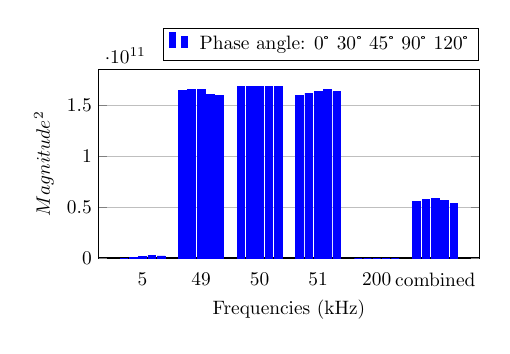
\begin{tikzpicture}[scale = 0.7]
          \begin{axis}[
              width  = 0.7*\textwidth,
              height = 5cm,
              major x tick style = transparent,
              ybar=2*\pgflinewidth,
              bar width=4pt,
              ymajorgrids = true,
              xlabel = {Frequencies (kHz)},
              ylabel = {$Magnitude^2$},
              symbolic x coords={5, 49, 50, 51, 200,combined},
              xtick = data,
              scaled x ticks = true,
              scaled y ticks = true,
              enlarge x limits=0.15,
              ymin=0,
              legend cell align=left,
              legend style={
                  at={(1,1.05)},
                  anchor=south east,
                  column sep=1ex
                },
              extra y ticks = 0.4,
              extra y tick labels={},
              extra y tick style={grid=major,major grid style={thick,draw=black}}
            ]
            \addplot[style={blue,fill=blue,mark=none}]
            coordinates {(5, 28165288) (49, 164300582087) (50, 167754581071) (51, 159204915664) (200, 19) (combined, 55316152356)
            };
        
             %\addplot[style={black,fill=red,mark=none}]
             %coordinates {(5, 27262976) (49, 164186030080) (50, 167786840064) (51, 159184322560) (200, 0)};
        
            \addplot[style={blue,fill=blue,mark=none}]
            coordinates {(5, 682813699) (49, 165638701140) (50, 167757951221) (51, 161622013902) (200, 6) (combined, 57679231120)
            };
        
            \addplot[style={blue,fill=blue,mark=none}]
            coordinates {(5, 1368984191) (49, 165006710536) (50, 167745947887) (51, 163313161637) (200, 14) (combined, 58261386167)
            };
        
            \addplot[style={blue,fill=blue,mark=none}]
            coordinates {(5, 2796749553) (49, 160349176237) (50, 167748444133) (51, 165437419087) (200, 19) (combined, 56341860579)
            };
        
            \addplot[style={blue,fill=blue,mark=none}]
            coordinates {(5, 2142148654) (49, 159011970308) (50, 167756010813) (51, 163022198679) (200, 29) (combined, 53976111895)
            };
        
            \legend{Phase angle: 0° 30° 45° 90° 120°}
            \addlegendimage{my legend}
          \end{axis}
        \end{tikzpicture}
        \caption{Sine waves}
        \label{fig:gf_sim_sine}
    \end{subfigure}

    %\vspace{0.5cm}
    
    \begin{subfigure}[b]{0.6\textwidth}
        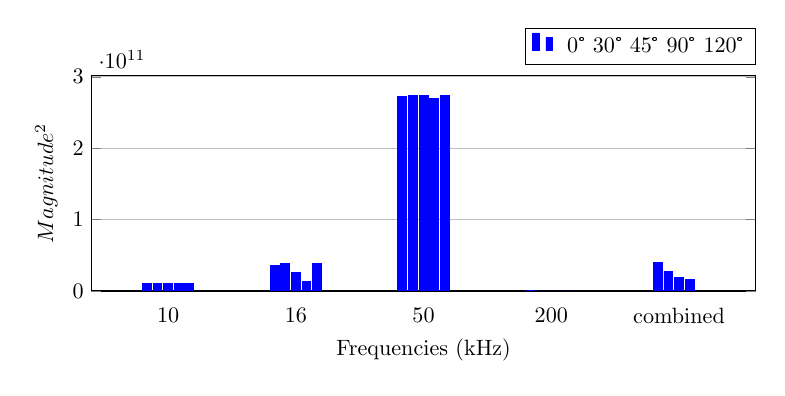
\begin{tikzpicture}[scale = 0.8]
          \begin{axis}[
              width  = \textwidth,
              height = 5cm,
              major x tick style = transparent,
              ybar=2*\pgflinewidth,
              bar width=4pt,
              ymajorgrids = true,
              xlabel = {Frequencies (kHz)},
              ylabel = {$Magnitude^2$},
              symbolic x coords={10, 16, 50, 200, combined},
              xtick = data,
              scaled x ticks = true,
              scaled y ticks = true,
              enlarge x limits=0.15,
              ymin=0,
              legend cell align=left,
              legend style={
                  at={(1,1.05)},
                  anchor=south east,
                  column sep=1ex
                },
              extra y ticks = 0.4,
              extra y tick labels={},
              extra y tick style={grid=major,major grid style={thick,draw=black}}
            ]
            \addplot[style={blue,fill=blue,mark=none}]
            coordinates {(10, 10967862060) (16, 35190107208) (50, 271780927294) (200, 268402689) 
            (combined, 39636235246)
            };
        
            \addplot[style={blue,fill=blue,mark=none}]
            coordinates {(10, 10967862060) (16, 38711007665) (50, 274196551495) (200, 0) (combined, 27759917661)
            };
        
            \addplot[style={blue,fill=blue,mark=none}]
            coordinates {(10, 10967862060) (16, 25835512141) (50, 274196551495) (200, 0) 
            (combined, 19477158285)
            };
        
            \addplot[style={blue,fill=blue,mark=none}]
            coordinates {(10, 10967862060) (16, 13709827575) (50, 269902108471) (200, 0) 
            (combined, 16577256943)
            };
        
            
            \addplot[style={blue,fill=blue,mark=none}]
            coordinates {(10, 10967862060) (16, 38711007665) (50, 274196551495) (200, 0) 
            %(combined, 6703613435)
            };
        
            \legend{0° 30° 45° 90° 120°}
            \addlegendimage{my legend}
          \end{axis}
        \end{tikzpicture}
        \caption{Rectangular waves}
    \end{subfigure}
    \hfill
    \begin{subfigure}[b]{0.35\textwidth}
        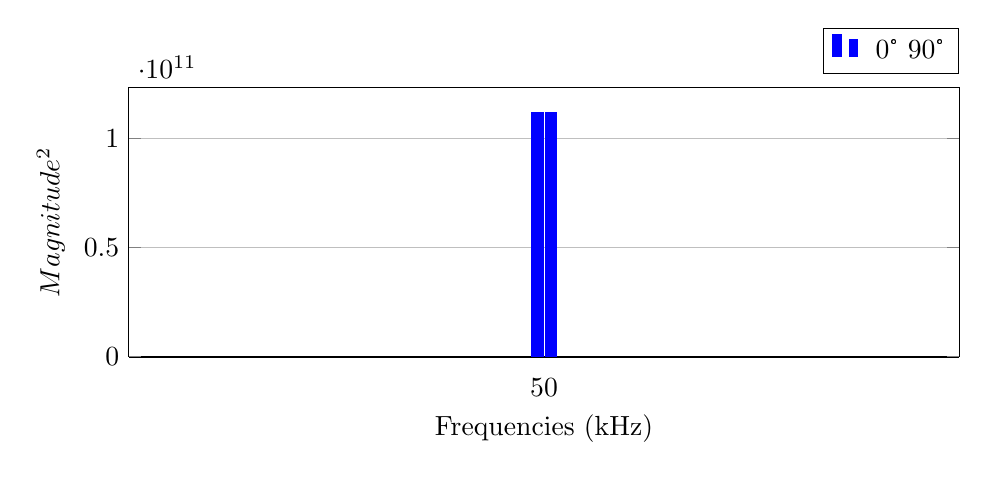
\begin{tikzpicture}
          \begin{axis}[
              width  = \textwidth,
              height = 5cm,
              major x tick style = transparent,
              ybar=2*\pgflinewidth,
              bar width=4pt,
              ymajorgrids = true,
              xlabel = {Frequencies (kHz)},
              ylabel = {$Magnitude^2$},
              symbolic x coords={50},
              xtick = data,
              scaled x ticks = true,
              scaled y ticks = true,
              enlarge x limits=0.15,
              ymin=0,
              legend cell align=left,
              legend style={
                  at={(1,1.05)},
                  anchor=south east,
                  column sep=1ex
                },
              extra y ticks = 0.4,
              extra y tick labels={},
              extra y tick style={grid=major,major grid style={thick,draw=black}}
            ]
            \addplot[style={blue,fill=blue,mark=none}]
            coordinates {(50, 112045721003)};
        
            \addplot[style={blue,fill=blue,mark=none}]
            coordinates {(50, 112045721002)};
        
            \legend{0° 90°}
            \addlegendimage{my legend}
          \end{axis}
        \end{tikzpicture}
        \caption{Triangle waves}
    \end{subfigure}
    
    \caption{Results of MATLAB simulation with floating-point numbers}
    \label{fig:gf_sim}
\end{figure}

The obtained result aligns with expectations, as the Goertzel filter exhibits a high magnitude response only for waves containing a component around 50 kHz, which corresponds to the signal frequency to detect ($F_k$).
As shown in Fig. n. \ref{fig:gf_sim_sine}, the filter in this design can barely differentiate between 49, 50 and 51 kHz signals. By changing the number of samples, we concluded that the frequency resolution is depending on the number of samples ($N$), as demonstrated that by the fact that, for example, when $N = 500$, the magnitudes for 50 kHz signals are much different from those for 49 and 51 kHz (Fig. n. \ref{fig:gf_sim_N500}), and the difference between those is much more recognizable.

\begin{figure}[H]
  \centering
  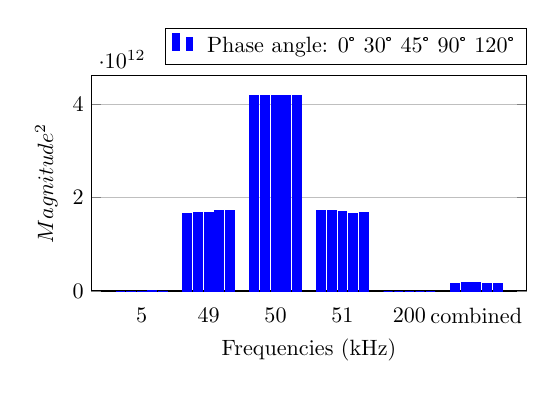
\begin{tikzpicture}[scale = 0.8]
    \begin{axis}[
        width  = 0.7*\textwidth,
        height = 5cm,
        major x tick style = transparent,
        ybar=2*\pgflinewidth,
        bar width=4pt,
        ymajorgrids = true,
        xlabel = {Frequencies (kHz)},
        ylabel = {$Magnitude^2$},
        symbolic x coords={5, 49, 50, 51, 200, combined},
        xtick = data,
        scaled x ticks = true,
        scaled y ticks = true,
        enlarge x limits=0.15,
        ymin=0,
        legend cell align=left,
        legend style={
            at={(1,1.05)},
            anchor=south east,
            column sep=1ex
          },
        extra y ticks = 0.4,
        extra y tick labels={},
        extra y tick style={grid=major,major grid style={thick,draw=black}}
      ]
      \addplot[style={blue,fill=blue,mark=none}]
      coordinates {(5, 28136055) (49, 1666618598937) (50, 4193875917772) (51, 1732388606682) (200, 205) 
      (combined, 167767402016)
      };

      \addplot[style={blue,fill=blue,mark=none}]
      coordinates {(5, 683029058) (49, 1674052576567) (50, 4193942960824) (51, 1725444346577) (200, 41) 
      (combined, 175769719174)
      };
  
      \addplot[style={blue,fill=blue,mark=none}]
      coordinates {(5, 1369507272) (49, 1689292248901) (50, 4193627387892) (51, 1710630899751) (200, 59) 
      (combined, 177898066729)
      };

      \addplot[style={blue,fill=blue,mark=none}]
      coordinates {(5, 2796634597) (49, 1733120151328) (50, 4193826613449) (51, 1667358625940) (200, 61) 
      (combined, 172045669337)
      };
  
      \addplot[style={blue,fill=blue,mark=none}]
      coordinates {(5, 2141985241) (49, 1725657357466) (50, 4193909153782) (51, 1674273740527) (200, 124) 
      (combined, 164047439042)
      };
  
      \legend{Phase angle: 0° 30° 45° 90° 120°}
      \addlegendimage{my legend}
    \end{axis}
  \end{tikzpicture}
    
  \caption{Results of MATLAB simulation of sine waves, N = 500}
  \label{fig:gf_sim_N500}
\end{figure}

The magnitudes of multi-tone waves with all the frequencies combined are lower than those of single-tone waves in 50 kHz. We suspect, this is due to the multi-tone waves are normalized to $0$ to $2^{14} - 1$, hence their components corresponding to 50 kHz is smaller than those single-tone waves.

\subsection{MATLAB Simulation with integers and LSB truncation}  \label{sec:matlab-int}

Since we aim to synthetize our VHDL implementation in real hardware and we aim to develop it in a way that is efficient in both performance and resources used, we analysed the difference between representing numbers as integers and as floating points.
To do so, we created another version of the Goertzel filter that used integers instead of floating-point numbers, with least significant bits (LSB) truncated to mimic what we would need to do in the VHDL implementation. The purpose of this version is to verify that any deviation between the MATLAB and VHDL results is attributed to the expected truncation error resulting from the filter design, rather than errors arising from mistakes in the VHDL implementation.
LSB are truncated as demonstrated in Fig. n. \ref{code:lsb_trunc}, where the value of $s(n)$ first divided by $2^{LSB\_TRUNC}$, next is passed to the \texttt{floor()} function, which converts the result of the expression inside to the nearest lower integer. The result is then multiplied by $2^{LSB\_TRUNC}$, effectively quantizing the result to 18 bits, as required by the specifications in Table n. \ref{tab:specifications}.

\lstset{language=Matlab}
\begin{figure}[H] \begin{lstlisting}
LSB_TRUNC = 5; % internal data's LSB truncated
...
s(n) = floor(double(signal(n) + multi_prod - sprev2) / 2 ^ LSB_TRUNC) * (2 ^ LSB_TRUNC);
\end{lstlisting}
\caption{Code snippet for LSB truncation}
\label{code:lsb_trunc}
\end{figure}

We compared the results of the two functions, as shown in Fig. n. \ref{fig:gf_sim_int} and Table \ref{tab:result}. The differences between the 2 versions is at most $1.2 \times 10^8$, and considering that the output is in the magnitude of $10^{11}$, the error is less than $0.1\%$, which can be considered acceptable in view of the reduced complexity given by avoiding floating numbers.
The outputs are again written into files and to be read by the VHDL testbench, which will be further discussed in Section n. \ref{sec:testbench}.

\begin{figure}[H]
  \centering
  \begin{subfigure}[b]{\textwidth}
    \centering
    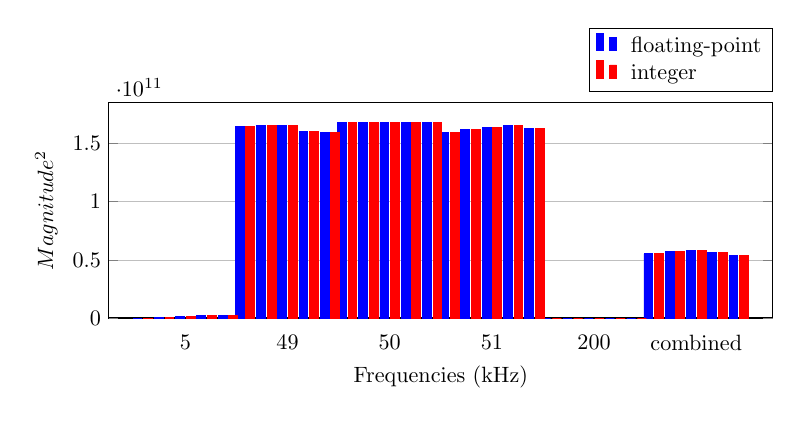
\begin{tikzpicture}[scale = 0.8]
      \begin{axis}[
          width  = \textwidth,
          height = 5cm,
          major x tick style = transparent,
          ybar=2*\pgflinewidth,
          bar width=4pt,
          ymajorgrids = true,
          xlabel = {Frequencies (kHz)},
          ylabel = {$Magnitude^2$},
          symbolic x coords={5, 49, 50, 51, 200, combined},
          xtick = data,
          scaled x ticks = true,
          scaled y ticks = true,
          enlarge x limits=0.15,
          ymin=0,
          legend cell align=left,
          legend style={
              at={(1,1.05)},
              anchor=south east,
              column sep=1ex
            },
          extra y ticks = 0.4,
          extra y tick labels={},
          extra y tick style={grid=major,major grid style={thick,draw=black}}
        ]
        \addplot[style={blue,fill=blue,mark=none}]
        coordinates {(5, 28165288) (49, 164300582087) (50, 167754581071) (51, 159204915664) (200, 19) (combined, 55316152356)};
        \addplot[style={red,fill=red,mark=none}]
        coordinates {(5, 27262976) (49, 164186030080) (50, 167786840064) (51, 159184322560) (200, 0) (combined, 55293509632)};
        \addplot[style={blue,fill=blue,mark=none}]
        coordinates {(5, 682813699) (49, 165638701140) (50, 167757951221) (51, 161622013902) (200, 6) (combined, 57679231120)};
        \addplot[style={red,fill=red,mark=none}]
        coordinates {(5, 679477248) (49, 165589024768) (50, 167845560320) (51, 161633796096) (200, 0) (combined, 57680068608)};
        \addplot[style={blue,fill=blue,mark=none}]
        coordinates {(5, 1368984191) (49, 165006710536) (50, 167745947887) (51, 163313161637) (200, 14) (combined, 58261386167)};
        \addplot[style={red,fill=red,mark=none}]
        coordinates {(5, 1365245952) (49, 165033279488) (50, 167784742912) (51, 163238117376) (200, 0) (combined, 58294534144)};
        \addplot[style={blue,fill=blue,mark=none}]
        coordinates {(5, 2796749553) (49, 160349176237) (50, 167748444133) (51, 165437419087) (200, 19) (combined, 56341860579)};
        \addplot[style={red,fill=red,mark=none}]
        coordinates {(5, 2791309312) (49, 160327270400) (50, 167723925504) (51, 165435932672) (200, 0) (combined, 56329502720)};
        \addplot[style={blue,fill=blue,mark=none}]
        coordinates {(5, 2142148654) (49, 159011970308) (50, 167756010813) (51, 163022198679) (200, 29) (combined, 53976111895)};
        \addplot[style={red,fill=red,mark=none}]
        coordinates {(5, 2139095040) (49, 159020744704) (50, 167832977408) (51, 163108093952) (200, 0) (combined, 53953429504)};
        \legend{floating-point, integer}
        \addlegendimage{my legend}
      \end{axis}
    \end{tikzpicture}
    \caption{Sine waves}
  \end{subfigure}


  \begin{subfigure}[b]{\textwidth}
  \centering
    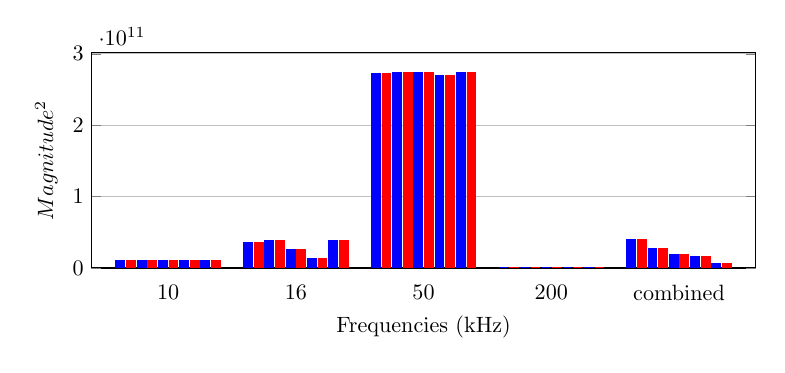
\begin{tikzpicture}[scale = 0.8]
      \begin{axis}[
          width  = \textwidth,
          height = 5cm,
          major x tick style = transparent,
          ybar=2*\pgflinewidth,
          bar width=4pt,
          ymajorgrids = true,
          xlabel = {Frequencies (kHz)},
          ylabel = {$Magnitude^2$},
          symbolic x coords={10, 16, 50, 200, combined},
          xtick = data,
          scaled x ticks = true,
          scaled y ticks = true,
          enlarge x limits=0.15,
          ymin=0,
          legend cell align=left,
          legend style={
              at={(1,1.05)},
              anchor=south east,
              column sep=1ex
            },
          extra y ticks = 0.4,
          extra y tick labels={},
          extra y tick style={grid=major,major grid style={thick,draw=black}}
        ]
        \addplot[style={blue,fill=blue,mark=none}]
        coordinates {(10, 10967862060) (16, 35190107208) (50, 271780927294) (200, 268402689) (combined, 39636235246)};
        \addplot[style={red,fill=red,mark=none}]
        coordinates {(10, 10951327744) (16, 35108421632) (50, 271730081792) (200, 266338304) (combined, 39696990208)};
        \addplot[style={blue,fill=blue,mark=none}]
        coordinates {(10, 10967862060) (16, 38711007665) (50, 274196551495) (200, 0) (combined, 27759917661)};
        \addplot[style={red,fill=red,mark=none}]
        coordinates {(10, 10984882176) (16, 38669385728) (50, 274141806592) (200, 0) (combined, 27736932352)};
        \addplot[style={blue,fill=blue,mark=none}]
        coordinates {(10, 10967862060) (16, 25835512141) (50, 274196551495) (200, 0) (combined, 19477158285)};
        \addplot[style={red,fill=red,mark=none}]
        coordinates {(10, 10974396416) (16, 25813843968) (50, 274080989184) (200, 0) (combined, 19480444928)};
        \addplot[style={blue,fill=blue,mark=none}]
        coordinates {(10, 10967862060) (16, 13709827575) (50, 269902108471) (200, 0) (combined, 16577256943)};
        \addplot[style={red,fill=red,mark=none}]
        coordinates {(10, 10982785024) (16, 13719568384) (50, 269859422208) (200, 0) (combined, 16571695104)};
        \addplot[style={blue,fill=blue,mark=none}]
        coordinates {(10, 10967862060) (16, 38711007665) (50, 274196551495) (200, 0) (combined, 6703613435)};
        \addplot[style={red,fill=red,mark=none}]
        coordinates {(10, 10970202112) (16, 38646317056) (50, 274141806592) (200, 0) (combined, 6696206336)};
      \end{axis}
    \end{tikzpicture}
    \caption{Rectangular waves}
  \end{subfigure}

  \vspace{0.5cm}

  \begin{subfigure}[b]{0.5\textwidth}
    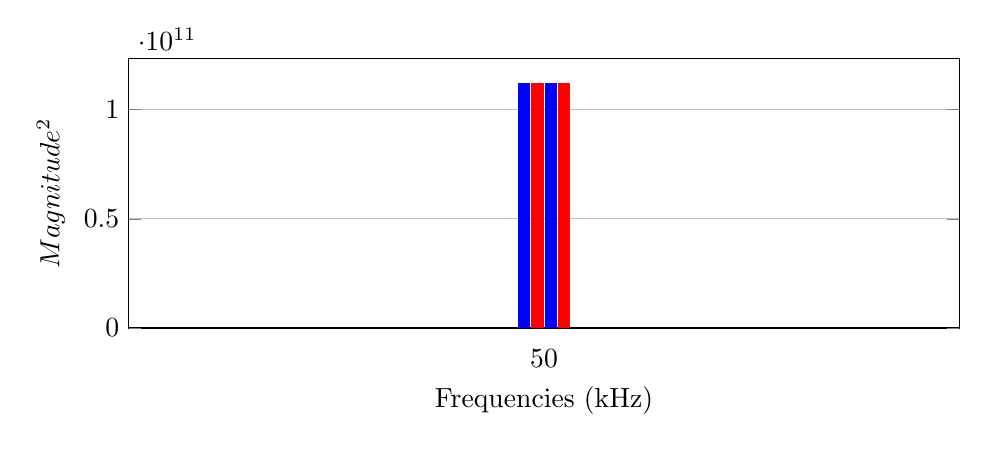
\begin{tikzpicture}
      \begin{axis}[
          width  = \textwidth,
          height = 5cm,
          major x tick style = transparent,
          ybar=2*\pgflinewidth,
          bar width=4pt,
          ymajorgrids = true,
          xlabel = {Frequencies (kHz)},
          ylabel = {$Magnitude^2$},
          symbolic x coords={50},
          xtick = data,
          scaled x ticks = true,
          scaled y ticks = true,
          enlarge x limits=0.15,
          ymin=0,
          legend cell align=left,
          legend style={
              at={(1,1.05)},
              anchor=south east,
              column sep=1ex
            },
          extra y ticks = 0.4,
          extra y tick labels={},
          extra y tick style={grid=major,major grid style={thick,draw=black}}
        ]
        \addplot[style={blue,fill=blue,mark=none}]
        coordinates {(50, 112045721003)};
        \addplot[style={red,fill=red,mark=none}]
        coordinates {(50, 112042442752)};
        \addplot[style={blue,fill=blue,mark=none}]
        coordinates {(50, 112045721002)};
        \addplot[style={red,fill=red,mark=none}]
        coordinates {(50, 112059219968)};
      \end{axis}
    \end{tikzpicture}
    \caption{Triangle waves}
  \end{subfigure}

  \caption{Results of MATLAB simulation with integers and LSB truncation}
  \label{fig:gf_sim_int}
\end{figure}


\section{Implementation}\label{sec:implementation}

We implemented the filter with the specifications summarized in table \ref{tab:specifications}. \\

%\begin{itemize}
 %   \item Input data: 14-bit unsigned, offset binary numbers
  %  \item Internal data: 18-bit signed
   % \item Output data in terms of $y(n)^2$
    %\item Sampling frequency ($F_s$): 1 MHz
    %\item Signal frequency to detect ($F_k$): 50 kHz
    %\item $N$ = 100
%\end{itemize}
\begin{table}[ht]
\centering
\begin{tabular}{|l|l|}
\hline
Input data                  & 14-bit unsigned, offset binary numbers  \\ \hline
Internal data               & 18-bit signed                      \\ \hline
Output data (in terms of $y(n)^2$) & 18-bit signed                \\ \hline
Sampling frequency ($F_s$)  & 1 MHz                              \\ \hline
Signal frequency to detect ($F_k$) & 50 kHz                             \\ \hline
N                           & 100                                \\ \hline
\end{tabular}
\caption{Specifications for the project}
\label{tab:specifications}
\end{table}

Following the discussions in Section \ref{sec:theory} and \ref{sec:pc}, from Equation n.\ref{eq:COEFF}, we calculated the constant $C$.

\begin{align*}
C &= 2\cos(\omega_0) = 2\cos\left(\frac{2\pi m}{N}\right) \\
&= 2\cos\left(\frac{2\pi F_k}{F_s}\right) \\
&= 2\cos\left(\frac{2\pi \times 50000}{1000000}\right) \approx 1.9021
\end{align*}

To use $C$ in our VHDL implementation, we rounded and converted it to an integer as following:

\lstset{language=VHDL}
\begin{figure}[H]\begin{lstlisting}
GENERIC (
    INT_BW : POSITIVE := 18;  -- bit width for internal data
    C : SIGNED(INT_BW - 1 DOWNTO 0) := "01" & x"E6F1";
    C_F : POSITIVE := INT_BW - 2 -- # of bits of fractional part of C
);
\end{lstlisting}
\caption{Code snippet for the definition of $C$}
\end{figure}

Here $C$ is represented in the code as a signed integer equals to $1E6F1_{16} = 124657$, and \texttt{C\_F} is used to represented that the fractional part of \texttt{C} are 16 bits, i.e. $C$ is rounded into:
\[
C = 124657 \times 2^{-16} = 1.9021148681640625
\]

\subsection{Port Description}

%The port employed by the Goertzel Filter is as following:\\
The following block diagram depicts the ports specified for our implementation of the Goertzel filter, with the corrisponding VHDL description in Fig. n. \ref{fig:vhdl_ports}.
% We need layers to draw the block diagram
\pgfdeclarelayer{background}
\pgfdeclarelayer{foreground}
\pgfsetlayers{background,main,foreground}
% Define a few styles and constants
\tikzstyle{sensor}=[draw, fill=blue!20, text width=5em, 
text centered, minimum height=2.5em]
\tikzstyle{ann} = [above, text width=6em]
\tikzstyle{naveqs} = [sensor, text width=6em, fill=white!20, 
minimum height=8em, rounded corners]
\def\blockdist{2.3}
\def\edgedist{1}
\begin{center}
    \begin{tikzpicture}[>={Latex[scale=1.5]}]
        %% Encoder
        \node (naveq) [naveqs] {goertzel};
        %% Inputs
        \draw[<-] ($(naveq.south west)!0.8!(naveq.north west)$) -- +(-\edgedist,0) node [left] {Clk\_CI};
        \draw[<-] ($(naveq.south west)!0.6!(naveq.north west)$) -- +(-\edgedist,0) node [left] {Rst\_RBI};
        \draw[<-] ($(naveq.south west)!0.4!(naveq.north west)$) -- +(-\edgedist,0) node [left] {Sample\_SI};
        \draw[<-] ($(naveq.south west)!0.2!(naveq.north west)$) -- +(-\edgedist,0) node [left] {En\_SI};
        %% Outputs
        \draw[->] ($(naveq.south east)!0.6!(naveq.north east)$) -- +(\edgedist,0) node [right] {Magnitude\_sq\_SO};
        \draw[->] ($(naveq.south east)!0.4!(naveq.north east)$) -- +(\edgedist,0) node [right] {Done\_SO};
    \end{tikzpicture}
\end{center}





\lstset{language=VHDL}
\begin{figure}[H]\begin{lstlisting}
ENTITY goertzel IS
    GENERIC (
        N : POSITIVE := 100;
        SIG_BW : POSITIVE := 14;
        INT_BW : POSITIVE := 18;
        LSB_TRUNC : POSITIVE := 5;
        MAG_TRUNC : POSITIVE := 11;
        C : SIGNED(INT_BW - 1 DOWNTO 0) := "01" & x"E6F1";
        C_F : POSITIVE := INT_BW - 2 -- # of bits of fractional part of C
    );
    PORT (
        Clk_CI : IN STD_LOGIC;
        Rst_RBI : IN STD_LOGIC;
        Sample_SI : IN UNSIGNED(SIG_BW - 1 DOWNTO 0);
        Magnitude_sq_SO : OUT SIGNED(INT_BW - 1 DOWNTO 0);
        En_SI : IN STD_LOGIC;
        Done_SO : OUT STD_LOGIC
    );
END ENTITY goertzel;
\end{lstlisting}
\caption{Code snippet for port definition}
\label{fig:vhdl_ports}
\end{figure}

We specified generics in order to parametrize the design as much as possible, to favor reuse and portability. The description of each generic and port is as follow:
\begin{itemize}
    \item \texttt{N}: number of samples.
    \item \texttt{SIG\_BW}: bit width for input signal.
    \item \texttt{INT\_BW}: bit width for internal data.
    \item \texttt{LSB\_TRUNC}: number of bit in internal data's LSB to be truncated to avoid overflow.
    \item \texttt{MSG\_TRUNC}: number of bit in final result (\texttt{Magnitude\_sq\_SO})'LSB to be truncated to avoid overflow.
    \item \texttt{Clk\_CI}: input, clock signal for input (\texttt{Sample\_SI}) and sequencial logic in the filter.
    \item \texttt{Rst\_RBI}: input, active-high synchronous reset signal for internal memory in the filter.
    \item \texttt{Sample\_SI}: input data, 14-bit unsigned, offset binary numbers (as specified in the requirements).
    \item \texttt{Magnitude\_sq\_SO}: output data, 18-bit signed, in terms of $y(n)^2 / 2^{21}$.
    \item \texttt{En\_SI}: input, enable signal for the filter, active high.
    \item \texttt{Done\_SO}: output, indicating the processing of the filter is finish. It keeps high for 1 clock cycle.
\end{itemize}

As already mentioned, the implementation includes generics that are parameterized for ease of use, e.g. \texttt{N} and \texttt{C}. It allows for easy customization of parameters for different sampling frequency, signal frequency to detect, and the number of samples. However, it is important to carefully choose the number of truncated bits \texttt{LSB\_TRUNC} and \texttt{MAG\_TRUNC} to avoid overflow. Simulation can help determine the maximum possible value of $s(n)$ and output, hence decide the number of bits required.

\subsection{Algorithm Implementation}
\label{sec:algo}
Following Fig n. \ref{fig:gf_overview} , we mapped the theoretical description of the algorithm into VHDL code.
From equation n. \ref{eq:UPDATE}, the calculation of $s(n)$ is mapped according to the following code snippet:

\lstset{language=VHDL}
\begin{figure}[H]\begin{lstlisting}
Sum <= resize(SIGNED('0' & Sample_SI), Sum'LENGTH) +
    resize(shift_right(C * s1_D, C_F - LSB_TRUNC), Sum'LENGTH) -
    shift_left(resize(s2_D, Sum'LENGTH), LSB_TRUNC);
s0 <= Sum(INT_BW + LSB_TRUNC - 1 DOWNTO LSB_TRUNC);
...
PROCESS (Clk_CI) BEGIN
    IF rising_edge(Clk_CI) THEN
        IF Rst_RBI = '1' THEN ... ELSE
            IF (Active_V = '1') THEN
                s1_D <= s0;
                s2_D <= s1_D;
            ELSE
                s1_D <= (OTHERS => '0');
                s2_D <= (OTHERS => '0');
            END IF;
            ...
        END IF;
    END IF;
END PROCESS;
\end{lstlisting}
\caption{Code snippet for the calculation of $s(n)$}
\end{figure}
Where:
\begin{itemize}
    \item \texttt{s0} = $s(n)$ from Equation n. \ref{eq:UPDATE}
    \item \texttt{s1} = $s(n-1)$ 
    \item \texttt{s2} = $s(n-2)$
\end{itemize}
Here $s(n)$ (\texttt{s0} in the code) is calculated by performing the following steps:
\begin{enumerate}
    \item The input signal, \texttt{Sample\_SI} is extended with a leading zero to match the length of \texttt{Sum}.
    \item The product of \texttt{C} and \texttt{s1\_D} is calculated and right-shifted by \texttt{(C\_F - LSB\_TRUNC)} bits using \texttt{shift\_right}, as \texttt{C\_F} bits of \texttt{C} is fractional part. The result is resized to match the length of \texttt{Sum}.
    \item The negative of \texttt{s2\_D} is resized to match the length of \texttt{Sum}.
    \item The three values calculated above are added (+) together and assigned to the \texttt{Sum} signal.
    \item \texttt{s0} is assigned the value of \texttt{Sum} from bit position \texttt{(INT\_BW + LSB\_TRUNC - 1)} down to bit position \texttt{LSB\_TRUNC}.
\end{enumerate}

We truncate \texttt{s0} because we use 18 bit for internal data, as specified in the specification, but that is not enough to store the result of $s(n)$. We discovered in our MATLAB simulation, as what will be introduced in Section n. \ref{sec:simulation}, that the the maximum value of $s(n)$ is between $2^{21}$ to $2^{22}$, while maximum value can be represented by a signed 18-bit integer is $2^{17} - 1$. To avoid overflow, we truncate 5 bits of LSB.

$y(n)$ (\texttt{Magnitude\_sq\_SO}) is calculated according to Equation n. \ref{eq:yn2}, which is demonstrated with the following code snippet:

\lstset{language=VHDL}
\begin{figure}[H]
\begin{lstlisting}
-- results has been shifted by 2*LSB_TRUNC = 10 bits
-- MATLAB sim shows that the results take at most 38 bits, hence truncate additional 11 bits (MAG_TRUNC) to fit into INT_BW (18 bits)
Magnitude_sq <= resize(shift_right(
    s1_D * s1_D +
    s2_D * s2_D -
    shift_right(s1_D * s2_D * C, C_F),
    MAG_TRUNC), Magnitude_sq'LENGTH);
...
PROCESS (Clk_CI) BEGIN
    IF rising_edge(Clk_CI) THEN
        ...
        Magnitude_sq_SO <= Magnitude_sq;
    END IF;
END PROCESS;
\end{lstlisting}
\caption{Code snippet for the calculation of $y(n)$}
\end{figure}

Similar to the calculation of $s(n)$, the product of (\texttt{1\_D * s2\_D * C, C\_F}) is first right-shifted by (\texttt{(C\_F - LSB\_TRUNC)}$\times 2$)  bits due to the fractional part of \texttt{C}.

The \texttt{MAG\_TRUNC} bits of the LSB in the intermediate result, obtained by calculating \texttt{(s1\_D * s1\_D + s2\_D * s2\_D - s1\_D * s2\_D * C, C\_F)}, are truncated. Similar to \texttt{s0}, MATLAB simulation showed that the maximum value of output is between $2^{37}$ and $2^{38}$, hence we truncate 21 bits of LSB of integral part. As the 5 bits of LSB of \texttt{s1\_D} and \texttt{s2\_D} are already truncated, we only need to truncate an additional 11 bits, as defined in \texttt{MAG\_TRUNC}.

In the design of the implementation, we have made a trade-off to truncate the bits instead of rounding them. This is because we can save the hardware source (e.g. area of silicon) that would be occupied by a rounding circuit. Additionally, the rounding of the last bit is often negligible and does not significantly affect the overall result: for the calculation of $s(n)$, the least significant bit (LSB) will be further truncated when we calculate the final result; as for the output calculation, the importance of result accuracy depends on the specific application. In some cases, the primary objective of the filter is to detect the presence of a signal rather than achieving high precision in the result.

It is worth-noting that bit shifting is performed using functions \texttt{shift\_left()} and \texttt{shift\_right()}, instead of \texttt{SRL}, \texttt{SLL}, \texttt{SRA}, and \texttt{SLA} operators. \texttt{SRL}, \texttt{SLL}, \texttt{SRA}, and \texttt{SLA} behave unexpectedly or incorrectly for different types, and hence be removed in IEEE Standard for VHDL Language Reference Manual (IEEE 1076). \cite{vhdlshift} \texttt{shift\_left()} and \texttt{shift\_right()} were introduced in VHDL-2008 with the \texttt{numeric\_std} library to be used with \texttt{UNSIGNED} and \texttt{SIGNED} types.

\subsection{Control Signals}

We includes two control signals: \texttt{En\_SI} and \texttt{Done\_SO} in the design, which serve specific purposes for ease of application and downstream circuit usage.

The \texttt{En\_SI} signal can be used to control the input data. For example, it can be used to indicate when the Analog-to-Digital Converter (ADC) starts producing valid output. Before \texttt{En\_SI} is high, the internal signals (e.g., \texttt{s1\_D}, \texttt{s2\_D}) are set to zero to ensure that when the filter starts to accept input data, the values in \texttt{s1\_D}, \texttt{s2\_D} are correct (i.e. equal to 0).

The \texttt{Done\_SO} signal indicates the completion of the calculation process, signaling that the filter has finished computing the output. This makes it easier for downstream circuits to utilize the output, for example, instructing when to load the result into a First-In-First-Out (FIFO) buffer for further processing. This functionality is achieved by employing a counter, \texttt{Cnt\_D}, and asserting the \texttt{Done\_SO} signal when the counter reaches the number of samples \texttt{N}.

\subsection{Timing Performance Consideration}

We also consider the timing performance of the filter.

First, it is improved by using Equation n. \ref{eq:yn2}, which utilizes \texttt{s1\_D} and \texttt{s2\_D}, instead of \texttt{s0} and \texttt{s1\_D}. This has effectively split the critical path in half, one being the calculation of \texttt{s0} and the other being that of \texttt{Magnitude\_sq\_SO}. This reduces the propagation delay and making it easier for EDA tools to meet timing requirements in place-and-route stage, and potentially allowing the circuit to be integrated in designs with a higher sampling frequency.

Second, The output result is loaded into a memory behind \texttt{Magnitude\_sq\_SO}, as described in Section n. \ref{sec:algo}. This may improve timing performance for driving high fanout or complex circuits from the output port; however it comes with a cost of the use of additional flip-flops, hence it is good for devices, like FPGA, which usually have sufficient flip-flops; however, for ASIC, it may not be a good idea, as it may increase the circuit area. The inclusion of this particular piece of code depends on the design platform and specific requirements of the project.




\subsection{Verification} \label{sec:testbench}

A VHDL testbench is used to verify the functional behaviour of the filter. Input signals and expected results, generated from the MATLAB simulation mentioned in Section n. \ref{sec:matlab-float} and \ref{sec:matlab-int}, are read from files. The file format used hexadecimal representation, with each line representing an entity and fixed-length fields for input and output values. The testbench read and converted the values \texttt{SIGNED} for comparison with the output of the filter under test. The verification flow is demonstrated in Code Snippet \ref{code:testbench}.
The output of the filter is compared with the expected results using \texttt{ASSERT} in VHDL, such that the verification can be done automatically, rather than with manually inspecting the waveforms. The results matched exactly, confirming the correctness of the implementation.

\lstset{language=VHDL}
\begin{figure}[H]
\begin{lstlisting}
FOR i IN TEST_CASE'RANGE LOOP
    -- open input signal file
    file_open(fstatus, fptr, INPUT_DIR & TEST_CASE(i), read_mode);
    WHILE (NOT endfile(fptr)) LOOP
        WAIT UNTIL Clk_CI = '1';
        En_SI <= '1';
        readline(fptr, file_line);
        hread(file_line, var_data);
        Sample_SI <= resize(var_data, Sample_SI'LENGTH);
    END LOOP;
    file_close(fptr);
    -- wait for DUT to finish
    En_SI <= '0';
    WAIT UNTIL Done_SO = '1';
    REPORT "Test case " & INTEGER'IMAGE(i) & ": " & TEST_CASE(i);
    -- open expected result file
    file_open(fstatus, fptr, EXPECTED_DIR & TEST_CASE(i), read_mode);
    WHILE (NOT endfile(fptr)) LOOP
        readline(fptr, file_line);
        hread(file_line, var_expected);

        ASSERT (resize(var_expected, Magnitude_sq_SO'LENGTH) = Magnitude_sq_SO)
        REPORT "FAIL, Expected Magnitude_sq_SO: " & INTEGER'IMAGE(to_integer(var_expected)) & " Actual: " & INTEGER'IMAGE(to_integer(Magnitude_sq_SO)) SEVERITY WARNING;
    END LOOP;
    file_close(fptr);
END LOOP;
\end{lstlisting}
\caption{\label{code:testbench}Code snippet for verification}
\end{figure}

\section{Conclusion}

In this project, we explored the Goertzel Filter as a digital signal processing algorithm for efficiently computing individual discrete Fourier transform (DFT) bins. The filter provides an alternative to the fast Fourier transform (FFT) for applications that require only a few frequency components, making it particularly useful for detecting specific frequencies in a signal. Our project focused on the design and implementation of a Goertzel Filter in VHDL, along with the development of a corresponding test bench.
The theoretical background of the Goertzel Algorithm was presented, explaining its principles and advantages. A comprehensive literature review was conducted to understand the state-of-the-art applications of the Goertzel Filter. Based on this knowledge, we proceeded with the implementation of the filter in VHDL, following the specified requirements. The implementation included a detailed description of the filter's ports, algorithm, control signals, and considerations for timing performance.
To validate the functionality and accuracy of our Goertzel Filter design, we conducted simulations using MATLAB and VHDL testbench. The MATLAB simulation with floating-point numbers allowed us to confirm our understanding of the Goertzel algorithm. Subsequently, we performed MATLAB simulations with integers and LSB truncation to verify that any deviation between MATLAB and VHDL results was due to the expected truncation error resulting from the filter design, rather than implementation mistakes in VHDL. The VHDL testbench provided further confirmation, as the results matched exactly with the MATLAB simulation, ensuring the correctness of our implementation.
In conclusion, our project successfully explored, designed, and implemented a Goertzel Filter in VHDL. Through thorough simulations and comparisons with MATLAB, we confirmed the accuracy and reliability of our implementation. The Goertzel Filter offers an efficient solution for frequency detection in various applications, and our work contributes to its understanding and practical implementation.
% \end{multicols}

%\section{References}
\bibliographystyle{unsrt}
\bibliography{bib} 

\newpage
\section{Appendix}
\appendix
\section{Results of Goertzel Filter simulation in MATLAB}
\pagenumbering{roman}
%\renewcommand{\thesection}{\Roman{section}}
\begin{table}[H]
  \begin{tabular}{|c c||c|c|c|}
    \hline
    \multicolumn{2}{|c||}{\bf Input signal} & \multirow{2}*{\bf Floating-point} & \multirow{2}*{\bf Integer} & \multirow{2}*{\bf Difference}             \\
    \textbf{Frequency (kHz)}                & \textbf{Phase (°)}                &                            &                               &           \\
    \hline
    \multicolumn{5}{|c|}{\bf Sine wave}                                                                                                                  \\
    \hline
    \multirow{5}*{5}                        & 0                                 & 28165288                   & 27262976                      & 902312    \\
                                            & 30                                & 682813699                  & 679477248                     & 3336451   \\
                                            & 45                                & 1368984191                 & 1365245952                    & 3738239   \\
                                            & 90                                & 2796749553                 & 2791309312                    & 5440241   \\
                                            & 120                               & 2142148654                 & 2139095040                    & 3053614   \\
    \hline
    \multirow{5}*{49}                       & 0                                 & 164300582087               & 164186030080                  & 114552007 \\
                                            & 30                                & 165638701140               & 165589024768                  & 49676372  \\
                                            & 45                                & 165006710536               & 165033279488                  & -26568952 \\
                                            & 90                                & 160349176237               & 160327270400                  & 21905837  \\
                                            & 120                               & 159011970308               & 159020744704                  & -8774396  \\
    \hline
    \multirow{5}*{50}                       & 0                                 & 167754581071               & 167786840064                  & -32258993 \\
                                            & 30                                & 167757951221               & 167845560320                  & -87609099 \\
                                            & 45                                & 167745947887               & 167784742912                  & -38795025 \\
                                            & 90                                & 167748444133               & 167723925504                  & 24518629  \\
                                            & 120                               & 167756010813               & 167832977408                  & -76966595 \\
    \hline
    \multirow{5}*{51}                       & 0                                 & 159204915664               & 159184322560                  & 20593104  \\
                                            & 30                                & 161622013902               & 161633796096                  & -11782194 \\
                                            & 45                                & 163313161637               & 163238117376                  & 75044261  \\
                                            & 90                                & 165437419087               & 165435932672                  & 1486415   \\
                                            & 120                               & 163022198679               & 163108093952                  & -85895273 \\
    \hline
    \multirow{5}*{200}                      & 0                                 & 19                         & 0                             & 19        \\
                                            & 30                                & 6                          & 0                             & 6         \\
                                            & 45                                & 14                         & 0                             & 14        \\
                                            & 90                                & 19                         & 0                             & 19        \\
                                            & 120                               & 29                         & 0                             & 29        \\
    \hline
    \multirow{5}*{combined}                 & 0                                 & 55316152356                & 55293509632                   & 22642724  \\
                                            & 30                                & 57679231120                & 57680068608                   & -837488   \\
                                            & 45                                & 58261386167                & 58294534144                   & -33147977 \\
                                            & 90                                & 56341860579                & 56329502720                   & 12357859  \\
                                            & 120                               & 53976111895                & 53953429504                   & 22682391  \\
    \hline
  \end{tabular}
\end{table}

\begin{table}[H]
  \begin{tabular}{|c c||c|c|c|}
    \hline
    \multicolumn{2}{|c||}{\bf Input signal} & \multirow{2}*{\bf Floating-point} & \multirow{2}*{\bf Integer} & \multirow{2}*{\bf Difference}             \\
    \textbf{Frequency (kHz)}                & \textbf{Phase (°)}                &                            &                               &           \\
    \hline
    \multicolumn{5}{|c|}{\bf Rectangular wave}                                                                                                           \\
    \hline
    \multirow{5}*{10}                       & 0                                 & 10967862060                & 10951327744                   & 16534316  \\
                                            & 30                                & 10967862060                & 10984882176                   & -17020116 \\
                                            & 45                                & 10967862060                & 10974396416                   & -6534356  \\
                                            & 90                                & 10967862060                & 10982785024                   & -14922964 \\
                                            & 120                               & 10967862060                & 10970202112                   & -2340052  \\
    \hline
    \multirow{5}*{16}                       & 0                                 & 35190107208                & 35108421632                   & 81685576  \\
                                            & 30                                & 38711007665                & 38669385728                   & 41621937  \\
                                            & 45                                & 25835512141                & 25813843968                   & 21668173  \\
                                            & 90                                & 13709827575                & 13719568384                   & -9740809  \\
                                            & 120                               & 38711007665                & 38646317056                   & 64690609  \\
    \hline
    \multirow{5}*{50}                       & 0                                 & 271780927294               & 271730081792                  & 50845502  \\
                                            & 30                                & 274196551495               & 274141806592                  & 54744903  \\
                                            & 45                                & 274196551495               & 274080989184                  & 115562311 \\
                                            & 90                                & 269902108471               & 269859422208                  & 42686263  \\
                                            & 120                               & 274196551495               & 274141806592                  & 54744903  \\
    \hline
    \multirow{5}*{200}                      & 0                                 & 268402689                  & 266338304                     & 2064385   \\
                                            & 30                                & 0                          & 0                             & 0         \\
                                            & 45                                & 0                          & 0                             & 0         \\
                                            & 90                                & 0                          & 0                             & 0         \\
                                            & 120                               & 0                          & 0                             & 0         \\
    \hline
    \multirow{5}*{combined}                 & 0                                 & 39636235246                & 39696990208                   & -60754962 \\
                                            & 30                                & 27759917661                & 27736932352                   & 22985309  \\
                                            & 45                                & 19477158285                & 19480444928                   & -3286643  \\
                                            & 90                                & 16577256943                & 16571695104                   & 5561839   \\
                                            & 120                               & 6703613435                 & 6696206336                    & 7407099   \\
    \hline
    \multicolumn{5}{|c|}{\bf Triangle wave}                                                                                                              \\
    \hline
    \multirow{2}*{50}                       & 0                                 & 112045721003               & 112042442752                  & 3278251   \\
                                            & 90                                & 112045721002               & 112059219968                  & -13498966 \\
    \hline
    % \caption{TEST}
    % \label{tab:goertzel_results}
  \end{tabular}
  \caption{\label{tab:result} Results of Goertzel Filter simulation in MATLAB}
\end{table}
\newpage
\section{Code of Goertzel Filter implementation in VHDL}

\lstset{language=VHDL}
\begin{lstlisting}

LIBRARY IEEE;
USE IEEE.STD_LOGIC_1164.ALL;
USE IEEE.NUMERIC_STD.ALL;
-- for constant calculation only (using clog2()), still synthesizable
USE IEEE.MATH_REAL.ALL;

ENTITY goertzel IS
    GENERIC (
        N         : POSITIVE := 100; -- Number of samples
        SIG_BW    : POSITIVE := 14;  -- bit width for input signal
        INT_BW    : POSITIVE := 18;  -- bit width for internal data
        LSB_TRUNC : POSITIVE := 5;   -- truncate internal data's LSB to avoid overflow
        MAG_TRUNC : POSITIVE := 11;  -- truncate final result (Magnitude_sq_SO)

        -- Coefficient for multiplication with s0 = 2cos(2pi Fk/Fs)
        --
        -- Sampling frequency (Fs) = 1 MHz
        -- Target frequency (Fk) = 50 kHz
        -- 2cos(2pi m/N) = 2cos(2pi Fk/Fs) = 2 * cos (2pi * 50E3 / 1E6) = 1.90211303259031
        -- 1.90211303259031 -> rounded to 1.9021148681640625 = 0x1E6F1 * 2^-16
        C : SIGNED(INT_BW - 1 DOWNTO 0) := "01" & x"E6F1";
        C_F : POSITIVE := INT_BW - 2 -- # of bits of fractional part of C
    );
    PORT (
        Clk_CI  : IN STD_LOGIC;
        Rst_RBI : IN STD_LOGIC;

        -- Signals
        -- offset binary numbers
        -- 1st sample should arrive the same clk cycle as the rising edge of En_SI
        Sample_SI : IN UNSIGNED(SIG_BW - 1 DOWNTO 0);

        -- output in terms of (magnitude^2 / 2^21)
        -- (maximum value of magnitude^2 is between 2^37 to 2^38)
        Magnitude_sq_SO : OUT SIGNED(INT_BW - 1 DOWNTO 0);

        -- Controls
        -- enable, active high
        En_SI : IN STD_LOGIC;
        -- active high, keep high for 1 clk cycle when finished
        Done_SO : OUT STD_LOGIC
    );
END ENTITY goertzel;

ARCHITECTURE behavioural OF goertzel IS

    -- for bit width calculation
    FUNCTION clog2(
        num : IN POSITIVE
    )
        RETURN POSITIVE IS
        VARIABLE num_in_log2 : POSITIVE;
    BEGIN
        num_in_log2 := POSITIVE(ceil(log2(REAL(num))));
        RETURN num_in_log2;
    END FUNCTION clog2;

    -- to count when the process finishes
    SIGNAL Cnt_D : UNSIGNED(clog2(N) - 1 DOWNTO 0) := (OTHERS => '0');
    -- state of the entity
    SIGNAL Active_D : STD_LOGIC := '0';

    -- intermediate result, delayed (z^-1) s0
    SIGNAL s0, s1_D, s2_D : SIGNED(INT_BW - 1 DOWNTO 0);

    -- Sum = Sample_SI + C * s2_D - s1_D
    SIGNAL Sum          : SIGNED(INT_BW + LSB_TRUNC - 1 DOWNTO 0);
    SIGNAL Magnitude_sq : SIGNED(INT_BW - 1 DOWNTO 0);

BEGIN
    -- calculate the intermediate result
    -- C: (INT_BW - C_F - 1 DOWNTO -C_F) -> (1 DOWNTO -16)
    -- s1_D: (INT_BW + LSB_TRUNC - 1 DOWNTO LSB_TRUNC -> 22 DOWNTO 5)
    -- product: ((INT_BW - C_F - 1) + (INT_BW + LSB_TRUNC - 1)) DOWNTO -C_F - (-LSB_TRUNC)) -> (23 DOWNTO -11)
    -- take interger part -> shift (C * s1_D) right by 11 bits (C_F - LSB_TRUNC)
    Sum <=
        resize(SIGNED('0' & Sample_SI), Sum'LENGTH) +
        resize(shift_right(C * s1_D, C_F - LSB_TRUNC), Sum'LENGTH) -
        shift_left(resize(s2_D, Sum'LENGTH), LSB_TRUNC);
    s0 <= Sum(INT_BW + LSB_TRUNC - 1 DOWNTO LSB_TRUNC);

    -- results has been shifted by 2*LSB_TRUNC = 10 bits
    -- MATLAB sim shows that the results take at most 38 bits, hence truncate additional 11 bits (MAG_TRUNC) to fit into INT_BW (18 bits)
    Magnitude_sq <= resize(shift_right(
        s1_D * s1_D +
        s2_D * s2_D -
        shift_right(s1_D * s2_D * C, C_F),
        MAG_TRUNC), Magnitude_sq'LENGTH);

    PROCESS (Clk_CI)
        VARIABLE Active_V : STD_LOGIC;
    BEGIN
        IF rising_edge(Clk_CI) THEN
            IF Rst_RBI = '1' THEN
                Cnt_D    <= (OTHERS => '0');
                Active_D <= '0';
                s1_D     <= (OTHERS => '0');
                s2_D     <= (OTHERS => '0');
                Done_SO  <= '0';
            ELSE
                Active_V := Active_D;
                Done_SO <= '0';
                Cnt_D   <= Cnt_D + 1;

                -- calculated starts
                IF (Active_V = '0' AND En_SI = '1') THEN
                    Active_V := '1';
                    Cnt_D <= (OTHERS => '0');
                END IF;

                -- store intermediate result
                IF (Active_V = '1') THEN
                    s1_D <= s0;
                    s2_D <= s1_D;
                ELSE
                    s1_D <= (OTHERS => '0');
                    s2_D <= (OTHERS => '0');
                END IF;

                -- check if calculation is finished
                -- N - 1 because:
                -- index of Cnt_D starts from 0 -> -1
                -- Cnt_D starts counting 2 clk cycles after 1st sample arrives -> -2
                -- downstream is fetching output 1 clk cycle before -> +1
                -- output to FF -> +1
                IF (Active_V = '1' AND Cnt_D = to_unsigned(N - 1, Cnt_D'LENGTH)) THEN
                    Active_V := '0';
                    Done_SO <= '1';
                END IF;

                Active_D <= Active_V;
            END IF;

            -- output to FF for better timing
            -- reset is unnecessary, as the output is guard by Done_SO, also save routing resource
            Magnitude_sq_SO <= Magnitude_sq;
        END IF;
    END PROCESS;
END behavioural;
\end{lstlisting}

\section{Code of VHDL testbench}

\lstset{language=VHDL}
\begin{lstlisting}
LIBRARY IEEE;
USE IEEE.STD_LOGIC_1164.ALL;
USE IEEE.NUMERIC_STD.ALL;
-- USE IEEE.MATH_REAL.ALL;
USE STD.TEXTIO.ALL;

ENTITY goertzel_tb IS
END goertzel_tb;

ARCHITECTURE testbench_arch OF goertzel_tb IS
    FUNCTION to_100_char(string_in : STRING) RETURN STRING IS
        VARIABLE V                     : STRING(1 TO 100) := (OTHERS => ' ');
    BEGIN
        IF string_in'length > 100 THEN
            RETURN string_in(1 TO 100);
        ELSE
            V(1 TO string_in'length) := string_in;
            RETURN V;
        END IF;
    END to_100_char;

    TYPE STRING_LIST IS ARRAY (NATURAL RANGE <>) OF STRING(1 TO 100);

    CONSTANT INPUT_DIR    : STRING      := "test_cases/input/";
    CONSTANT EXPECTED_DIR : STRING      := "test_cases/expected/";
    CONSTANT TEST_CASE    : STRING_LIST := (
        to_100_char("sine_wave_50kHz_0deg.txt" & NUL),
        to_100_char("sine_wave_50kHz_30deg.txt" & NUL),
        to_100_char("sine_wave_50kHz_45deg.txt" & NUL),
        to_100_char("sine_wave_50kHz_90deg.txt" & NUL),
        to_100_char("sine_wave_50kHz_120deg.txt" & NUL),
        to_100_char("sine_wave_49kHz_0deg.txt" & NUL),
        to_100_char("sine_wave_49kHz_30deg.txt" & NUL),
        to_100_char("sine_wave_49kHz_45deg.txt" & NUL),
        to_100_char("sine_wave_49kHz_90deg.txt" & NUL),
        to_100_char("sine_wave_49kHz_120deg.txt" & NUL),
        to_100_char("sine_wave_51kHz_0deg.txt" & NUL),
        to_100_char("sine_wave_51kHz_30deg.txt" & NUL),
        to_100_char("sine_wave_51kHz_45deg.txt" & NUL),
        to_100_char("sine_wave_51kHz_90deg.txt" & NUL),
        to_100_char("sine_wave_51kHz_120deg.txt" & NUL),
        to_100_char("sine_wave_5kHz_0deg.txt" & NUL),
        to_100_char("sine_wave_5kHz_30deg.txt" & NUL),
        to_100_char("sine_wave_5kHz_45deg.txt" & NUL),
        to_100_char("sine_wave_5kHz_90deg.txt" & NUL),
        to_100_char("sine_wave_5kHz_120deg.txt" & NUL),
        to_100_char("sine_wave_200kHz_0deg.txt" & NUL),
        to_100_char("sine_wave_200kHz_30deg.txt" & NUL),
        to_100_char("sine_wave_200kHz_45deg.txt" & NUL),
        to_100_char("sine_wave_200kHz_90deg.txt" & NUL),
        to_100_char("sine_wave_200kHz_120deg.txt" & NUL),
        to_100_char("sine_wave_combined_0deg.txt" & NUL),
        to_100_char("sine_wave_combined_30deg.txt" & NUL),
        to_100_char("sine_wave_combined_90deg.txt" & NUL),
        to_100_char("sine_wave_combined_120deg.txt" & NUL),
        to_100_char("sine_wave_combined_45deg.txt" & NUL),
        to_100_char("rectangular_wave_50kHz_0deg.txt" & NUL),
        to_100_char("rectangular_wave_50kHz_30deg.txt" & NUL),
        to_100_char("rectangular_wave_50kHz_45deg.txt" & NUL),
        to_100_char("rectangular_wave_50kHz_90deg.txt" & NUL),
        to_100_char("rectangular_wave_50kHz_120deg.txt" & NUL),
        to_100_char("rectangular_wave_16kHz_0deg.txt" & NUL),
        to_100_char("rectangular_wave_16kHz_30deg.txt" & NUL),
        to_100_char("rectangular_wave_16kHz_45deg.txt" & NUL),
        to_100_char("rectangular_wave_16kHz_90deg.txt" & NUL),
        to_100_char("rectangular_wave_16kHz_120deg.txt" & NUL),
        to_100_char("rectangular_wave_10kHz_0deg.txt" & NUL),
        to_100_char("rectangular_wave_10kHz_30deg.txt" & NUL),
        to_100_char("rectangular_wave_10kHz_45deg.txt" & NUL),
        to_100_char("rectangular_wave_10kHz_90deg.txt" & NUL),
        to_100_char("rectangular_wave_10kHz_120deg.txt" & NUL),
        to_100_char("rectangular_wave_200kHz_0deg.txt" & NUL),
        to_100_char("rectangular_wave_200kHz_30deg.txt" & NUL),
        to_100_char("rectangular_wave_200kHz_45deg.txt" & NUL),
        to_100_char("rectangular_wave_200kHz_90deg.txt" & NUL),
        to_100_char("rectangular_wave_200kHz_120deg.txt" & NUL),
        to_100_char("rectangular_wave_combined_0deg.txt" & NUL),
        to_100_char("rectangular_wave_combined_30deg.txt" & NUL),
        to_100_char("rectangular_wave_combined_45deg.txt" & NUL),
        to_100_char("rectangular_wave_combined_90deg.txt" & NUL),
        to_100_char("rectangular_wave_combined_120deg.txt" & NUL),
        to_100_char("triangle_wave_50kHz_0deg.txt" & NUL),
        to_100_char("triangle_wave_50kHz_90deg.txt" & NUL)
    );

    -- for File I/O
    CONSTANT SIG_LINE_BW : POSITIVE := 16; -- SIG_BW, rounded up to nearest multiple of 4
    CONSTANT EXP_LINE_BW : POSITIVE := 20;

    -- (clock period / 2) in simulation time
    CONSTANT CLK_T : TIME := 10 ns;

    -- for simulation
    SIGNAL Eof     : STD_LOGIC := '0';
    SIGNAL Sigterm : STD_LOGIC := '0';

    -- for DUT
    CONSTANT N             : POSITIVE                    := 100;
    CONSTANT SIG_BW        : POSITIVE                    := 14;
    CONSTANT INT_BW        : POSITIVE                    := 18;
    CONSTANT LSB_TRUNC     : POSITIVE                    := 5;
    CONSTANT MAG_TRUNC     : POSITIVE                    := 11;
    CONSTANT C             : SIGNED(INT_BW - 1 DOWNTO 0) := "01" & x"E6F1";
    CONSTANT C_F           : POSITIVE                    := INT_BW - 2;
    SIGNAL Clk_CI          : STD_LOGIC                   := '0';
    SIGNAL Rst_RBI         : STD_LOGIC                   := '0';
    SIGNAL Sample_SI       : UNSIGNED(SIG_BW - 1 DOWNTO 0);
    SIGNAL Magnitude_sq_SO : SIGNED(INT_BW - 1 DOWNTO 0);
    SIGNAL En_SI           : STD_LOGIC;
    SIGNAL Done_SO         : STD_LOGIC;

    -- File I/O
    FILE fptr : text;

    COMPONENT goertzel IS
        GENERIC (
            N         : POSITIVE                    := 100;
            SIG_BW    : POSITIVE                    := 14;
            INT_BW    : POSITIVE                    := 18;
            LSB_TRUNC : POSITIVE                    := 5;
            MAG_TRUNC : POSITIVE                    := 11;
            C         : SIGNED(INT_BW - 1 DOWNTO 0) := "01" & x"E6F1";
            C_F       : POSITIVE                    := INT_BW - 2
        );
        PORT (
            Clk_CI          : IN STD_LOGIC;
            Rst_RBI         : IN STD_LOGIC;
            Sample_SI       : IN UNSIGNED(SIG_BW - 1 DOWNTO 0);
            Magnitude_sq_SO : OUT SIGNED(INT_BW - 1 DOWNTO 0);
            En_SI           : IN STD_LOGIC;
            Done_SO         : OUT STD_LOGIC
        );
    END COMPONENT;

BEGIN

    ClockGenerator : PROCESS
    BEGIN
        clkloop : LOOP
            WAIT FOR CLK_T;
            Clk_CI <= NOT Clk_CI;
            IF Sigterm = '1' THEN
                EXIT;
            END IF;
        END LOOP clkloop;
        WAIT;
    END PROCESS;

    Rst_RBI <= '1', '0' AFTER 100 ns;

    GetData_proc : PROCESS

        VARIABLE fstatus : file_open_status;

        VARIABLE file_line    : line;
        VARIABLE var_data     : UNSIGNED(SIG_LINE_BW - 1 DOWNTO 0);
        VARIABLE var_expected : SIGNED(EXP_LINE_BW - 1 DOWNTO 0);
    BEGIN

        -- initialize

        var_data     := (OTHERS => '0');
        var_expected := (OTHERS => '0');
        Eof       <= '0';
        Sample_SI <= (OTHERS => '0');
        En_SI     <= '0';
        WAIT UNTIL Rst_RBI = '0';

        FOR i IN TEST_CASE'RANGE LOOP
            -- open input signal file
            file_open(fstatus, fptr, INPUT_DIR & TEST_CASE(i), read_mode);

            WHILE (NOT endfile(fptr)) LOOP
                WAIT UNTIL Clk_CI = '1';
                En_SI <= '1';
                readline(fptr, file_line);
                hread(file_line, var_data); -- hex
                Sample_SI <= resize(var_data, Sample_SI'LENGTH);
            END LOOP;

            file_close(fptr);

            -- wait for DUT to finish
            En_SI <= '0';
            WAIT UNTIL Done_SO = '1';
            REPORT "Test case " & INTEGER'IMAGE(i) & ": " & TEST_CASE(i);

            -- open expected result file
            file_open(fstatus, fptr, EXPECTED_DIR & TEST_CASE(i), read_mode);
            readline(fptr, file_line);
            hread(file_line, var_expected); -- hex

            ASSERT (resize(var_expected, Magnitude_sq_SO'LENGTH) = Magnitude_sq_SO)
            REPORT "FAIL, Expected Magnitude_sq_SO: " & INTEGER'IMAGE(to_integer(var_expected)) & " Actual: " & INTEGER'IMAGE(to_integer(Magnitude_sq_SO)) SEVERITY WARNING;

            file_close(fptr);
        END LOOP;

        -- terminate
        WAIT UNTIL rising_edge(Clk_CI);
        Eof     <= '1';
        Sigterm <= '1';
        WAIT;
    END PROCESS;

    DUT : goertzel
    GENERIC MAP(
        N         => N,
        SIG_BW    => SIG_BW,
        INT_BW    => INT_BW,
        LSB_TRUNC => LSB_TRUNC,
        MAG_TRUNC => MAG_TRUNC,
        C         => C,
        C_F       => C_F
    )
    PORT MAP(

        Clk_CI          => Clk_CI,
        Rst_RBI         => Rst_RBI,
        Sample_SI       => Sample_SI,
        Magnitude_sq_SO => Magnitude_sq_SO,
        En_SI           => En_SI,
        Done_SO         => Done_SO
    );
END testbench_arch;

\end{lstlisting}

\section{Code of MATLAB simulation}

\lstset{language=Matlab}
\begin{lstlisting}
% 1. Define constants
Fs = 1e6; % sampling frequency
Fk = 50e3; % frequency to detect
N = 100; % number of samples
INPUT_BIT_LEN = 14; % number of input bit length
INPUT_SWING = 14; % swing of input signal
INT_BIT_LEN = 18; % number of internal bit length

% VHDL impelmentation related
% bit width of COEFF due to internal data bit width limitation
% 18 - 2 = 16 bits for fractional part
COEFF_BW = INT_BIT_LEN - 2;
LSB_TRUNC = 5; % internal data's LSB truncated, as implemented in VHDL
MAG_TRUNC = 11; % truncate final result (magnitude^2)

% 2. Generate the waveforms
t = (0:N-1) / Fs;
phase_angles = [0, 30, 45, 90, 120];
% phase_angles = [0];

% Sine Waves
frequencies_sine = [50e3, 49e3, 51e3, 5e3, 200e3];
sine_waves = zeros(length(frequencies_sine), length(phase_angles), N, "int32");
sine_waves_combined_single = zeros(length(phase_angles), N, "single");
sine_waves_combined = zeros(length(phase_angles), N, "int32");

for i = 1:length(frequencies_sine)
    for j = 1:length(phase_angles)
        frequency = frequencies_sine(i);
        phase = phase_angles(j);
        sine_wave = sin(2*pi*frequency*t + deg2rad(phase));
        sine_waves(i, j, :) = scaleToInt(sine_wave, INPUT_BIT_LEN, INPUT_SWING);
        sine_waves_combined_single(j, :) = sine_waves_combined_single(j, :) + sine_wave / length(frequencies_sine);
    end
end

for j = 1:length(phase_angles)
    phase = phase_angles(j);
    sine_waves_combined(j, :) = scaleToInt(sine_waves_combined_single(j, :), INPUT_BIT_LEN, INPUT_SWING);
end

% Rectangular Waves
frequencies_rectangular = [50e3, 16e3, 10e3, 200e3];
rectangular_waves = zeros(length(frequencies_rectangular), length(phase_angles), N);
rectangular_waves_combined_single = zeros(length(phase_angles), N, "single");
rectangular_waves_combined = zeros(length(phase_angles), N, "int32");

for i = 1:length(frequencies_rectangular)
    for j = 1:length(phase_angles)
        frequency = frequencies_rectangular(i);
        phase = phase_angles(j);
        rectangular_wave = square(2*pi*frequency*t + deg2rad(phase));
        rectangular_waves(i, j, :) = scaleToInt(rectangular_wave, INPUT_BIT_LEN, INPUT_SWING);
        rectangular_waves_combined_single(j, :) = rectangular_waves_combined_single(j, :) + rectangular_wave / length(frequencies_rectangular);
    end
end

for j = 1:length(phase_angles)
    phase = phase_angles(j);
    rectangular_waves_combined(j, :) = scaleToInt(rectangular_waves_combined_single(j, :), INPUT_BIT_LEN, INPUT_SWING);
end

% Triangle Waves
phase_angles_triangle = [0, 90];
triangle_waves = zeros(length(phase_angles_triangle), N);

for i = 1:length(phase_angles_triangle)
    phase = phase_angles_triangle(i);
    triangle_wave = sawtooth(2*pi*50e3*t + deg2rad(phase), 0.5);
    triangle_waves(i, :) = scaleToInt(triangle_wave, INPUT_BIT_LEN, INPUT_SWING);
end

% 3. Goertzel Filter
sine_waves_dft = zeros(length(frequencies_sine), length(phase_angles), "int32");
for i = 1:length(frequencies_sine)
    for j = 1:length(phase_angles)
        dft_input = reshape(sine_waves(i, j, :), 1, []);
        magnitude_sq = goertzel_filter(dft_input, Fk, Fs);
        magnitude_sq_trunc = goertzel_filter_int(dft_input, Fk, Fs, COEFF_BW, LSB_TRUNC, MAG_TRUNC);
        sine_waves_dft(i, j) = magnitude_sq_trunc;
        fprintf("SIN freq: %d phase: %d mag: %.0f %d\n", frequencies_sine(i), phase_angles(j), magnitude_sq, magnitude_sq_trunc * 2 ^ (LSB_TRUNC * 2 + MAG_TRUNC));
    end
end

sine_waves_combined_dft = zeros(length(phase_angles), 1, "int32");
for i = 1:length(phase_angles)
    dft_input = reshape(sine_waves_combined(i, :), 1, []);
    magnitude_sq = goertzel_filter(dft_input, Fk, Fs);
    magnitude_sq_trunc = goertzel_filter_int(dft_input, Fk, Fs, COEFF_BW, LSB_TRUNC, MAG_TRUNC);
    sine_waves_combined_dft(i) = magnitude_sq_trunc;
    fprintf("SIN_COMB phase: %d mag: %.0f %d\n", phase_angles(i), magnitude_sq, magnitude_sq_trunc * 2 ^ (LSB_TRUNC * 2 + MAG_TRUNC));
end

rectangular_waves_dft = zeros(length(frequencies_rectangular), length(phase_angles), "int32");
for i = 1:length(frequencies_rectangular)
    for j = 1:length(phase_angles)
        dft_input = reshape(rectangular_waves(i, j, :), 1, []);
        magnitude_sq = goertzel_filter(dft_input, Fk, Fs);
        magnitude_sq_trunc = goertzel_filter_int(dft_input, Fk, Fs, COEFF_BW, LSB_TRUNC, MAG_TRUNC);
        rectangular_waves_dft(i, j) = magnitude_sq_trunc;
        fprintf("RECT freq: %d phase: %d mag: %.0f %d\n", frequencies_rectangular(i), phase_angles(j), magnitude_sq, magnitude_sq_trunc * 2 ^ (LSB_TRUNC * 2 + MAG_TRUNC));
    end
end

rectangular_waves_combined_dft = zeros(length(phase_angles), 1, "int32");
for i = 1:length(phase_angles)
    dft_input = reshape(rectangular_waves_combined(i, :), 1, []);
    magnitude_sq = goertzel_filter(dft_input, Fk, Fs);
    magnitude_sq_trunc = goertzel_filter_int(dft_input, Fk, Fs, COEFF_BW, LSB_TRUNC, MAG_TRUNC);
    rectangular_waves_combined_dft(i) = magnitude_sq_trunc;
    fprintf("RECT_COMB phase: %d mag: %.0f %d\n", phase_angles(i), magnitude_sq, magnitude_sq_trunc * 2 ^ (LSB_TRUNC * 2 + MAG_TRUNC));
end

triangle_waves_dft = zeros(length(phase_angles_triangle), 1, "int32");
for i = 1:length(phase_angles_triangle)
    dft_input = reshape(triangle_waves(i, :), 1, []);
    magnitude_sq = goertzel_filter(dft_input, Fk, Fs);
    magnitude_sq_trunc = goertzel_filter_int(dft_input, Fk, Fs, COEFF_BW, LSB_TRUNC, MAG_TRUNC);
    triangle_waves_dft(i) = magnitude_sq_trunc;
    fprintf("TRI phase: %d mag: %.0f %d\n", phase_angles_triangle(i), magnitude_sq, magnitude_sq_trunc * 2 ^ (LSB_TRUNC * 2 + MAG_TRUNC));
end

% 4. Output the waveforms to a file
% each entity occupies a row in the file

% Create folders
mkdir test_cases/input
mkdir test_cases/expected

% Fixed width and padding with zeros
% in hex format, hence /4
sigLineWidth = ceil(INPUT_BIT_LEN / 4);
targetLineWidth = 5;

% Loop through input signals & DFT results, and write each waveform to a separate file
filePrefix = 'sine_wave';
for i = 1:length(frequencies_sine)
    for j = 1:length(phase_angles)
        nameFreq = sprintf('%.0f%sHz', frequencies_sine(i) / 10^(3 * floor(log10(abs(frequencies_sine(i)))/3)), suffix(frequencies_sine(i)));

        fileName = sprintf('test_cases/input/%s_%s_%ddeg.txt', filePrefix, nameFreq, phase_angles(j));
        write_to_file(reshape(sine_waves(i, j, :), 1, []), fileName, sigLineWidth);

        fileName = sprintf('test_cases/expected/%s_%s_%ddeg.txt', filePrefix, nameFreq, phase_angles(j));
        write_to_file(reshape(sine_waves_dft(i, j, :), 1, []), fileName, targetLineWidth);
    end
end

filePrefix = 'sine_wave_combined';
for i = 1:length(phase_angles)
    fileName = sprintf('test_cases/input/%s_%ddeg.txt', filePrefix, phase_angles(i));
    write_to_file(sine_waves_combined(i, :), fileName, sigLineWidth);

    fileName = sprintf('test_cases/expected/%s_%ddeg.txt', filePrefix, phase_angles(i));
    write_to_file(sine_waves_combined_dft(i, :), fileName, targetLineWidth);
end

filePrefix = 'rectangular_wave';
for i = 1:length(frequencies_rectangular)
    for j = 1:length(phase_angles)
        nameFreq = sprintf('%.0f%sHz', frequencies_rectangular(i) / 10^(3 * floor(log10(abs(frequencies_rectangular(i)))/3)), suffix(frequencies_rectangular(i)));

        fileName = sprintf('test_cases/input/%s_%s_%ddeg.txt', filePrefix, nameFreq, phase_angles(j));
        write_to_file(reshape(rectangular_waves(i, j, :), 1, []), fileName, sigLineWidth);

        fileName = sprintf('test_cases/expected/%s_%s_%ddeg.txt', filePrefix, nameFreq, phase_angles(j));
        write_to_file(reshape(rectangular_waves_dft(i, j, :), 1, []), fileName, targetLineWidth);
    end
end

filePrefix = 'rectangular_wave_combined';
for i = 1:length(phase_angles)
    fileName = sprintf('test_cases/input/%s_%ddeg.txt', filePrefix, phase_angles(i));
    write_to_file(rectangular_waves_combined(i, :), fileName, sigLineWidth);

    fileName = sprintf('test_cases/expected/%s_%ddeg.txt', filePrefix, phase_angles(i));
    write_to_file(rectangular_waves_combined_dft(i, :), fileName, targetLineWidth);
end

filePrefix = 'triangle_wave';
for i = 1:length(phase_angles_triangle)
    fileName = sprintf('test_cases/input/%s_50kHz_%ddeg.txt', filePrefix, phase_angles_triangle(i));
    write_to_file(triangle_waves(i, :), fileName, sigLineWidth);

    fileName = sprintf('test_cases/expected/%s_50kHz_%ddeg.txt', filePrefix, phase_angles_triangle(i));
    write_to_file(triangle_waves_dft(i, :), fileName, targetLineWidth);
end

% 99. Function definitions in a script must appear at the end of the file

function output = scaleToInt(input, bit_len, input_swing)
    % Scale the waveforms to the range of 2^(bit_len - 1) +/- 2^input_swing
    scaled = (2 ^ bit_len - 1) / 2 + input * (2 ^ input_swing - 1) / 2;
    % Convert the scaled waveforms to (bit_len)-bit unsigned integers
    output = int32(round(scaled));
end

% Function to generate SI unit suffix
function s = suffix(num)
    units = {'', 'k', 'M', 'G', 'T', 'P', 'E'};
    exponent = log10(abs(num));
    exponent = floor(exponent / 3);
    exponent = max(min(exponent, numel(units)-1), 0);
    s = units{exponent+1};
end

function magnitude_sq = goertzel_filter(signal, targetFrequency, samplingRate)
    N = length(signal); % Length of the signal
    k = round(N * targetFrequency / samplingRate); % Bin frequency
    w = 2 * pi * k / N; % Angular frequency
    cosine = cos(w);
    coefficient = 2 * cosine;

    s = zeros(N, 1); % First intermediate variable
    sprev = 0; % Previous s[n-1]
    sprev2 = 0; % Previous s[n-2]

    % Iterate through the signal
    for n = 1:N
        s(n) = signal(n) + coefficient * sprev - sprev2;
        sprev2 = sprev;
        sprev = s(n);
    end

    % Compute the magnitude
    sN = s(N);
    sNprev = s(N-1);
    magnitude_sq = double(sN^2 + sNprev^2 - sN * sNprev * coefficient);
end

function magnitude_sq_trunc = goertzel_filter_int(signal, targetFrequency, samplingRate, coeffBw, lsbTrunc, magTrunc)
    N = length(signal); % Length of the signal
    k = round(N * targetFrequency / samplingRate); % Bin frequency
    w = 2 * pi * k / N; % Angular frequency
    cosine = cos(w);
    coefficient = 2 * cosine;
    % round acconding to coeffBw
    coefficient = convergent(coefficient * 2 ^ coeffBw) / (2 ^ coeffBw);

    s = zeros(N, 1); % First intermediate variable
    sprev = 0; % Previous s[n-1]
    sprev2 = 0; % Previous s[n-2]

    % Iterate through the signal
    for n = 1:N
        % truncate according to lsbTrunc
        multi_prod = floor(coefficient * sprev);
        % remove LSB instead of rounding, hence floor() instead of convergent()
        s(n) = floor(double(signal(n) + multi_prod - sprev2) / 2 ^ lsbTrunc) * (2 ^ lsbTrunc);

        sprev2 = sprev;
        sprev = s(n);
    end

    % Compute the magnitude
    sN = s(N);
    sNprev = s(N-1);
    magnitude_sq = double(sN^2 + sNprev^2 - sN * sNprev * coefficient);
    % take the integer part of (sN * sNprev * coefficient) only
    bit_shift = lsbTrunc * 2 + magTrunc;
    magnitude_sq_trunc = floor(magnitude_sq / 2 ^ bit_shift);
end

function write_to_file(signal, fileName, lineWidth)
    % Open the file for writing
    fileID = fopen(fileName, 'w');

    % Write each entity of the sine_wave to a line in the file
    for k = 1:length(signal)
        % dec2hex() can handle negative numbers
        fprintf(fileID, '%s\n', dec2hex(signal(k), lineWidth));
    end

    % Close the file
    fclose(fileID);
end
\end{lstlisting}


\end{document}




